\documentclass[
%parspace, % Add vertical space between paragraphs
%noindent, % No indentation of first lines in each paragraph
%nohyp, % No hypenation of words
%twoside, % Double sided format
%draft, % Quicker draft compilation (also disables images and hyperref links!)
%final, % Set final to hide todos
]{elteiktdk}[2024/04/26]

 \usepackage{tikz}
 \usetikzlibrary{positioning, arrows.meta, fit}

% The minted package is also supported for source highlighting
%\usepackage[newfloat]{minted}

% Document's metadata
\title{Conformalized Mean Curvature Flow with Walk on Spheres}
\date{2026}

% Author(s)' metadata
\author{Nagy Levente}
\degree{Computer Science BSc}
\period{III. grade}

% Superivsor(s)' metadata
\supervisor{Dr. Fábián Gábor}
\affiliation{Assistant Professor}

% University's metadata
\university{Eötvös Loránd University}
\faculty{Faculty of Informatics}
\department{Department of Numerical Analysis}
\city{Budapest}
\logo{elte_cimer_szines}

% Add bibliography file
\addbibresource{elteiktdk.bib}

% The document
\begin{document}
	
	% Set document language
	%\documentlang{hungarian}
	\documentlang{english}
	
	% List of todos (not in the final document)
	%\listoftodos[\todolabel]
	%\cleardoublepage
	
	% Cover and title page (mandatory)
	\makecover
	\cleardoublepage
	\maketitle
	
	% Table of contents (mandatory)
	\tableofcontents
	\cleardoublepage
	
	\begin{abstract}
		Partial differential equations (PDEs) play an important role in geometry processing, where their efficient numerical solution remains a significant challenge. Traditional numerical methods, such as finite element and finite difference methods, rely on spatial discretization and often require solving large, sparse linear systems, which can be computationally expensive. Walk on Spheres (WoS) methods offer an alternative approach by solving PDEs through stochastic sampling, without requiring a global spatial discretization or linear system solve. While classical WoS methods are primarily designed for fixed volumetric domains, recent developments have extended them to PDEs defined on embedded surfaces. In this work, we investigate a further extension to geometric evolution equations, focusing on the conformalized mean curvature flow (cMCF). This flow deforms genus-zero surfaces towards a spherical configuration while preserving their conformal structure and avoiding the singularities associated with standard mean curvature flow. We develop a stochastic formulation for solving cMCF using the Projected Walk on Spheres framework. By employing a semi-implicit time discretization and the delta tracking technique, we transform each time step into a screened Poisson problem that can be addressed using stochastic sampling, despite its spatially varying screening coefficient. We establish the theoretical framework for this approach and investigate its numerical implementation, discussing the challenges arising from the evolution of the underlying surface and the possible emergence of self-intersections. Our work demonstrates a potential extension of grid-free stochastic PDE solvers to geometric evolution problems.
	\end{abstract}
	
	% =====================================================================
	% 1. INTRODUCTION
	% =====================================================================
	\chapter{Introduction}
	\label{ch:intro}
	
	In this paper, we lay the groundwork for solving the conformalized mean-curvature flow (cMCF) with stochastic methods. In recent years, stochastic methods for solving partial differential equations (PDEs), such as the Walk on Spheres (WoS) method and its variants, have gained popularity in geometry processing because of their computational advantages. Unlike classical numerical PDE solvers such as the finite element or finite difference methods, they do not require solving large, sparse linear systems, which can be expensive in both time and memory. They need no volumetric mesh, so they avoid the problems caused by poor-quality discretizations; they can evaluate the solution at individual points, and they are trivially parallelizable. The cMCF itself, however, is defined on a surface mesh, so in our setting the quality of the mesh still matters.
	
	The objective of this work is to investigate whether such stochastic methods can be extended to geometric evolution equations, specifically to the cMCF. The cMCF is a geometric flow that deforms genus-zero surfaces towards a round sphere while avoiding the singularities of the regular mean curvature flow. Unlike conventional elliptic problems, which are defined on a fixed domain, geometric evolution equations introduce an additional challenge: the domain itself changes over time, so in general a numerical method must also account for the evolving geometry on which the equation is defined. For the cMCF, this can be avoided. Its operator is defined with respect to the metric of the initial surface, so the walks can be kept on the fixed original surface $S_0$, and only the embedding $\Phi$ is updated.
	
	We develop a stochastic formulation of the cMCF based on the WoS framework. Our results show that it is feasible to solve this flow with a stochastic PDE solver. However, maintaining the quality of the triangulation during the flow remains a challenge. In particular, the noise of the Monte Carlo estimates produces thin and flipped (inverted) triangles, which may affect the accuracy and stability of the subsequent steps. Since conventional WoS methods do not have to deal with mesh quality, this difficulty is specific to the present application.
	
	We also evaluate two simple strategies against mesh degeneration, a cyclic time step and a few final iterations with decreasing time steps, and outline directions for further research. Our primary contribution is to show that WoS-type solvers can be extended beyond fixed-domain problems to geometric flows whose operator is defined on a fixed reference surface, such as the cMCF.
	
	
	% =====================================================================
	% 2. BACKGROUND AND RELATED WORK  (short; everything else is introduced
	%    just in time, where it is first needed)
	% =====================================================================
	\chapter{Background and related work}
	\label{ch:background}
	
	In this chapter, we introduce the fundamental concepts and mathematical tools used throughout this work, and review the relevant background and related literature.
	
	\section{Preliminaries and notation}
	\label{sec:notation}
	
	\begin{definition}[Laplace operator]
		Let $\Omega \subset \mathbb{R}^d$ $(d \in \mathbb{N}^+)$ be a bounded domain, $u: \Omega \rightarrow \mathbb{R}$, $u \in C^2$. The Laplace operator in Cartesian coordinates is:
		\begin{equation}
			\Delta u = \nabla \cdot \nabla u = \sum^d_{i=1} \frac{\partial^2 u}{\partial x_i^2}
		\end{equation}
		
	\end{definition}
	
	\begin{definition}[Screened Poisson equation]
		\label{screenedPoi}
		Let $\Omega \subset \mathbb{R}^d$ $(d \in \mathbb{N}^+)$ be a bounded domain, $u: \Omega \rightarrow \mathbb{R}$, $u \in C^2$, $\sigma \geq 0$ a constant screening coefficient, $f$ an arbitrary source function and $g$ the boundary values. The screened Poisson equation with Dirichlet boundary conditions is
		\begin{equation}
			\begin{cases}
				\Delta u(x) - \sigma u(x) = -f(x), & x \in \Omega, \\
				u(x) = g(x), & x \in \partial \Omega 
			\end{cases}
		\end{equation}   
	\end{definition}
	
	\begin{remark}
		In the case of $\sigma = 0$, we get a simple \textit{Poisson equation} $\Delta u = -f$, and if $f = 0$ as well, we get the \textit{Laplace equation} $\Delta u = 0$.
	\end{remark}

	\begin{definition}[Green's function]
		Let $\Omega \subset \mathbb{R}^d$ $(d \in \mathbb{N^+})$ be a bounded domain.
		The Green's function $G: \Omega \times \Omega \rightarrow
		\mathbb{R}$ associated with the Laplace operator is defined by
		\begin{equation}
			\begin{cases}
				-\Delta_x G(x,y) = \delta_y(x),
				& x \in \Omega,\\
				G(x,y) = 0,
				& x \in \partial\Omega,
			\end{cases}
		\end{equation}
		where $\delta_y$ denotes the Dirac delta distribution (not to be confused with the time step $\delta$ used later)
		centered at $y \in \Omega$.
	\end{definition}

	\begin{definition}[Surface and immersion] 
		Let \(M\) be a compact, connected, two-dimensional smooth manifold without boundary (a closed surface), and let
		\[
		\Phi:M\to\mathbb{R}^3
		\]
		be a smooth immersion. In the experiments presented in this paper, \(M\) is assumed to be homeomorphic to the sphere \(S^2\), i.e.\ a surface of genus zero.
	\end{definition}
	
	\begin{definition}[Induced metric]
		The metric induced by $\Phi$ is the pullback of the Euclidean inner product,
		\begin{equation}
			(g_\Phi)_{ij} = \partial_i\Phi\cdot\partial_j\Phi ,
		\end{equation}
		where $\partial_i$ are derivatives with respect to local coordinates on~$M$.
	\end{definition}
	
	For a time-dependent family $\Phi_t$ we write $g_t$ for the metric induced
	by $\Phi_t$, and $\det g_t$ for its determinant in local coordinates.
	The area element of the surface is $dA_t = \sqrt{\det g_t}\,dx^1 dx^2$.
	
	\begin{definition}[Laplace--Beltrami operator]
		\label{lb}
		For a metric $g$ and a smooth function $f$ on $M$,
		\begin{equation}
			\Delta_g f = \frac{1}{\sqrt{\det g}}\,
			\partial_i\!\left(\sqrt{\det g}\; g^{ij}\partial_j f\right).
		\end{equation}
	\end{definition}

	
	\section{Walk on Spheres}
	
	Partial differential equations in geometry processing are traditionally solved
	with mesh- or grid-based numerical methods, such as the finite element or
	finite difference method. These methods discretize the whole domain, which is
	expensive in both time and memory, and their accuracy depends on the quality of
	the discretization: a poor mesh (for example one with badly shaped or
	degenerate elements) directly introduces error into
	the solution.   
	 
	\emph{Walk on Spheres} (WoS) avoids this. The method goes back to
	\textcite{10.1214/aoms/1177728169}, and was brought to
	geometry processing by \textcite{Sawhney:2020:MCG}. It needs no volumetric
	mesh and no global linear solve. To estimate the solution at a point $x$,
	consider a ball $B_r(x)$ with center $x$ and radius $r$ fully contained within the domain.
	The equation
	\begin{equation} \label{screenedPoissonIntegral}
		u(x) = \frac{c_r}{\left|\partial B_r(x)\right|}\int_{\partial B_r(x)} u(y) \, dy + \int_{B_r(x)} f(z)G^{\sigma}_r(x,z) \, dz
	\end{equation}
	holds for the screened Poisson equation, where $\left|\partial B_r(x)\right|$ is the area of the sphere $\partial B_r(x)$, $G^{\sigma}_r$ is the Green's function of the operator $\Delta-\sigma$ on the ball $B_r(x)$ (its free-space counterpart is the \textit{Yukawa potential}), and $c_r \le 1$ is the total weight of the boundary term, which accounts for the screening. For the Poisson equation ($\sigma = 0$) we have $c_r = 1$, and $G_r$ is the Green's function of the Laplacian on the ball. For the Laplace equation ($f = 0$), the second integral vanishes, since all information comes from the boundary.
	
	\begin{figure}[H]
		\centering
		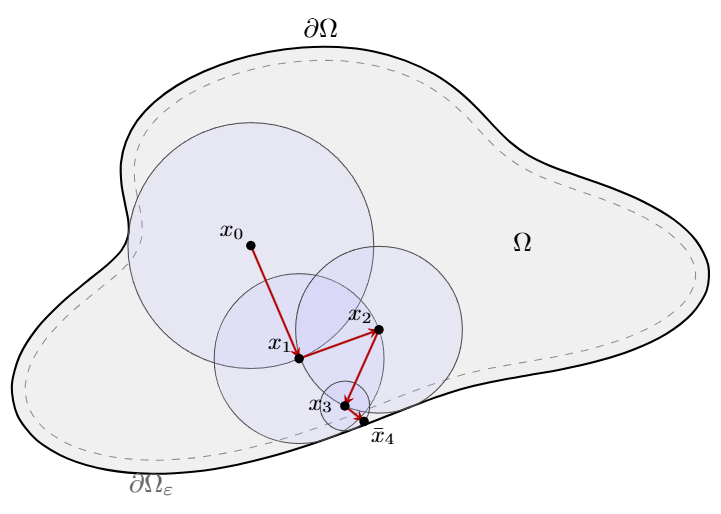
\includegraphics[scale=0.5]{images/wos_example.png}
		\caption{An example of a single walk from a point in the case of a Laplace equation. $\Omega$ is the inside of the domain, $\partial \Omega$ is the boundary, and $\partial \Omega_\epsilon$ is the $\epsilon$-range to the boundary, which also acts as hitting the boundary. $x_0$ is the initial starting point and $\overline{x}_4$ is the point where we terminated the walk. In the case of a Poisson equation, we also take a sample $y_k$ inside the balls $B_r(x_k)$}
		\label{fig:wos_example}
	\end{figure}
	
	Equation~\eqref{screenedPoissonIntegral} leads to the following algorithm. We start many walks from a point $x_0$. Each walk repeatedly jumps to a random point on the largest ball around its current position, collects the source contributions along the way, and terminates when it gets $\epsilon$-close to the boundary, where it reads the boundary value. The average of the walks is an estimate of $u(x_0)$. For the Laplace equation with Dirichlet boundary conditions, \textit{Kakutani's principle} states that
	\begin{equation}
		u(x) = \mathbb{E}\left[g(W_\tau)\right],
	\end{equation}
	where $W$ is a Brownian motion (Wiener process) started at $x$, and $\tau$ is its first exit time from $\Omega$. The \textit{mean value property} \cite{axler2001harmonic} states that
	\begin{equation}
		u(x) = \frac{1}{|\partial B_r(x)|}\int_{\partial B_r(x)} u(y) \, dy
	\end{equation}
	This property is the core of the method, and it appears as the first term of Equation~\eqref{screenedPoissonIntegral}. The estimator at a point $x_0$ is
	\begin{equation}
		u(x_0) = \frac{1}{N} \sum_{i=1}^{N} \widehat{u_f}(x_0)
	\end{equation} 
	where $N$ is the number of walks, and for the screened Poisson equation with Dirichlet boundary conditions, a single walk $\widehat{u}^{(i)}_f$ is defined recursively by
	
	\begin{equation}
		\widehat{u}_f(x_k) :=
		\begin{cases}
			g(\overline{x}_k), & x_k \in \partial\Omega_\epsilon \\
			c_r \widehat{u}_f(x_{k+1}) + \underbrace{\left| B_r(x_k) \right| f (y_k) G^{\sigma}_r(x_k, y_k)}_{\text{Poisson part}}, & \text{otherwise.}
		\end{cases}
	\end{equation}
	where $y_k\sim\mathcal U(B_r(x_k))$ and $\overline{x}_k$ is the boundary point closest to $x_k$. Instead of using the weight $c_r$, the walk can also be continued with probability $c_r$ and terminated with zero contribution otherwise (Russian roulette). The variance can be reduced further by sampling $y_k$ from a density proportional to $G^\sigma_r$ (importance sampling). Using the \textit{Feynman--Kac} formula, the solution of the screened Poisson equation can be written as
	\begin{equation}
		u(x) = \mathbb{E}\left[e^{-\sigma\tau} g(X_{\tau}) + \int_0^{\tau} e^{-\sigma t} f(X_t) \, dt\right]
	\end{equation}
	where $X_t = x + \sqrt{2}\,W_t$ is a Brownian motion whose generator is $\Delta$ (the standard Wiener process has generator $\frac{1}{2}\Delta$).
	
	\section{Walk on Spheres on surfaces}
	
	Classical WoS solves PDEs on volumetric domains in Euclidean space, whereas
	we need to solve a PDE on a two-dimensional surface embedded in
	$\mathbb{R}^3$. \textcite{Sugimoto:2024:PWoS} introduced \emph{Projected Walk
	on Spheres} (PWoS), which adapts WoS to surfaces using the closest point
	method: the walk takes ordinary WoS steps in $\mathbb{R}^3$ and projects every
	sample back to the surface.
	
	To make the projection well-defined, the sphere radius must be small enough
	that the closest point on the surface is unique inside the ball. For this, the
	algorithm first builds a medial axis point cloud of the surface, which gives a
	local feature size $\mathrm{lfs}$ at every point. A walk then proceeds as follows:
	\begin{enumerate}
		\item Start from a point $x_0$ on the surface.
		\item Take the largest admissible sphere around $x_k$, with radius $r_k$
		given by the distance to the nearest medial axis point (and, if there is a
		Dirichlet boundary, the distance to it, whichever is smaller).
		\item Sample a point $y_k$ uniformly on the sphere $\partial B_{r_k}(x_k)$ and, if needed, points inside the ball for the source term.
		\item Project it back to the surface, $x_{k+1} = \mathrm{cp}_S(y_k)$.
		\item Repeat steps 2--4 until the walk gets within $\epsilon$ of the Dirichlet
		boundary, or is terminated by Russian roulette.
	\end{enumerate}
	
	\begin{figure}[H]
		\begin{subfigure}{0.5\textwidth}
			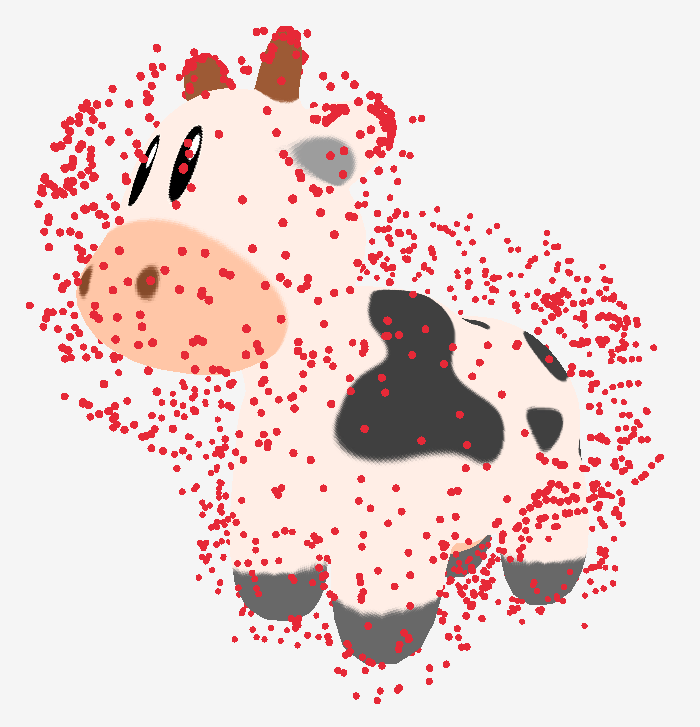
\includegraphics[scale=0.4]{images/medialaxispointcloudoutside.png}
			\caption{Medial axis points outside of the surface}
			\label{fig:medialaxispointcloudoutside}
		\end{subfigure}
		\begin{subfigure}{0.5\textwidth}
			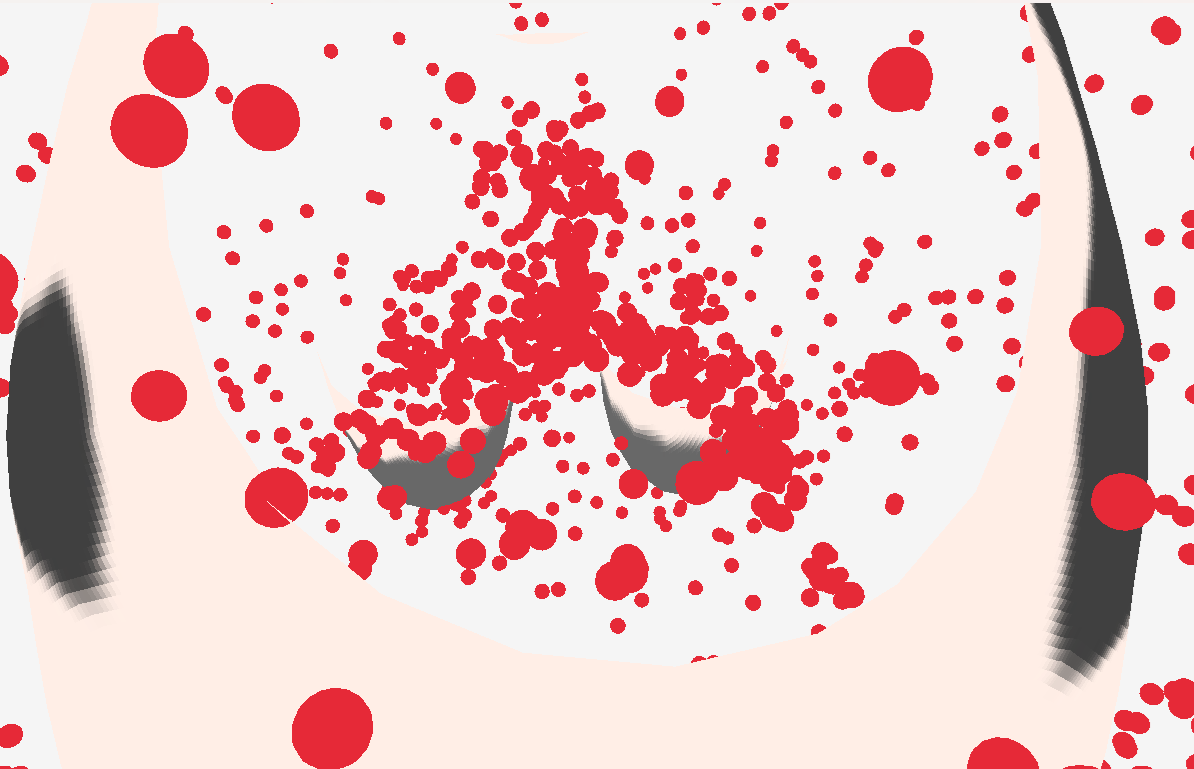
\includegraphics[scale=0.25]{images/medialaxispointcloudinside.png}
			\caption{Medial axis points inside the surface}
			\label{fig:medialaxispointcloudinside}
		\end{subfigure}
		\caption[Medial axis point cloud of Spot]{Medial axis point cloud of Spot \cite{crane2013robust} (10\,000 points).}
	\end{figure}
	
	\begin{remark}
		We do not discuss the construction of the medial axis point cloud in detail; it is described by \textcite{Sugimoto:2024:PWoS}.
	\end{remark}
	
	% =====================================================================
	% 3. THE FLOW
	% =====================================================================
	\chapter{Conformalized Mean-Curvature Flow}
	\label{ch:cmcf}
	
	\section{Regular Mean-Curvature Flow}
	
	Mean curvature flow can be thought of as a flow that pushes a point on a surface towards the average positions of its neighbors. This flow have the effect of smoothing the geometry.
	
	\begin{definition}[MCF]
		Let $M$ be a two-dimensional manifold, let $\Phi_t: M \rightarrow \mathbb{R}^3$ be a smooth family of immersions, and let $g_t(\cdot,\cdot)$ be the metric induced by the immersions at time $t$. We say that $\Phi_t$ is a solution to the mean-curvature flow if:
		\begin{equation}
			\frac{\partial \Phi_t}{\partial t} = \Delta_t \Phi_t
		\end{equation}
		where $\Delta_t$ is the Laplace-Beltrami operator \ref{lb} defined with respect to $g_t$.
	\end{definition}
	
	\section{Conformalization of the flow}
	\label{sec:cmcf-def}
	
	\textcite{kazhdan2012nonsingular} showed that the mean curvature flow can be made non-singular by a modification called conformalization.
	
	\begin{definition}[cMCF]
		Let $(M,h)$ be a two-dimensional Riemann manifold, let $\Phi_t: M \rightarrow \mathbb{R}^3$ be a smooth family of immersions, and let $g_t(\cdot,\cdot)$ be a metric induced by the immersion at time $t$, and also let us assume that in this case $h = g_0$. We then say that $\Phi_t$ is a solution to the conformalized mean curvature flow if:
		\begin{equation}
			\label{cMFC}
			\frac{\partial\Phi_t}{\partial t} = \sqrt{\left| g_t^{-1} g_0\right|}\Delta_{g_0}\Phi_t
		\end{equation}
		where $\Delta_{g_0}$ is the Laplace-Beltrami operator with respect to $g_0$.
	\end{definition}
	
	\begin{remark}
		For brevity, let
		\begin{equation}
			\label{alpha}
			\alpha(x,t) = \sqrt{\left| g_t^{-1} g_0\right|}, \qquad \Delta := \Delta_{g_0}
		\end{equation}
	\end{remark}	
	 
	\begin{remark}
		$\alpha(x,t)$ is the ratio of the initial and the current area element at $x$:
	\end{remark}
	
	\begin{equation}
		\label{alphaaa}
		\alpha(x,t) = \sqrt{\left| g_t^{-1} g_0\right|} = \sqrt{\frac{\det g_0}{\det g_t}} = \frac{\sqrt{\det g_0}}{\sqrt{\det g_t}} = \frac{dA_0}{dA_t}
	\end{equation}
	
	\section{Why cMCF?}
	
	Using the basic MCF introduces numerical instabilities while transforming the model, resulting in singularities.
	
	\begin{figure}[H]
		\centering
		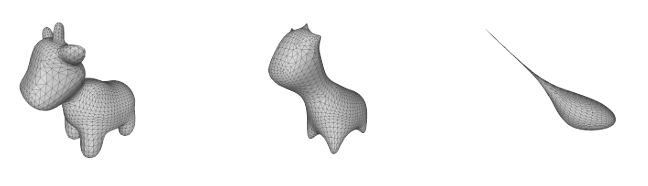
\includegraphics[scale=0.8]{images/spotbad.png}
		\caption{Regular mean-curvature flow pinches the neck of Spot, resulting in a singularity. Picture from: \textcite{wong2020application}}
		\label{fig:badspot}
	\end{figure}
	The cMCF avoids these singularities (Figure~\ref{fig:goodspot}) by using the fixed initial metric $g_0$ in the Laplace--Beltrami operator, together with the factor $\alpha(x,t)$ from Equation~\eqref{alpha}.
	
	\begin{figure}[H]
		\centering
		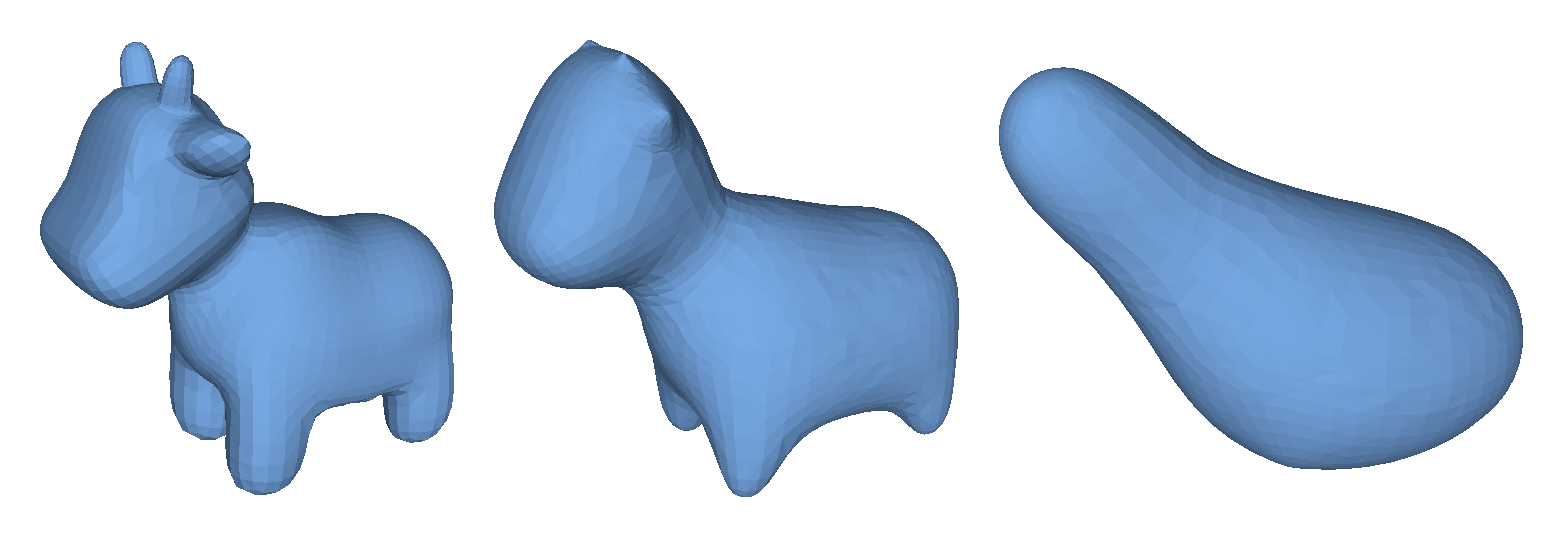
\includegraphics[scale=0.25]{images/spotgood.png}
		\caption{Conformalized mean-curvature flow avoids pinching the neck of Spot.}
		\label{fig:goodspot}
	\end{figure}
	
	
	% =====================================================================
	% 4. METHOD
	% =====================================================================
	\chapter{Solving cMCF with Walk on Spheres}
	\label{ch:method}
	
	\section{Idea}
	
	Using the notation of Equation~\eqref{alpha}, Equation~\eqref{cMFC} is a heat equation with a diffusivity that varies in space and time:
	
	\begin{equation}
		\label{heat}
		\frac{\partial \Phi_t}{\partial t} = \alpha(x,t)\Delta_{g_0}\Phi_t
	\end{equation}
	\textcite{zhou2026gridfree} recently proposed a WoS method for the inhomogeneous heat equation, but only with a constant diffusivity, whereas in our case the diffusivity $\alpha(x,t)$ varies in space and time; the authors mention non-constant diffusivity as future work. Instead of developing such a method, we discretize the equation in time and solve a sequence of elliptic problems. Since the operator of the cMCF is defined with respect to the fixed reference metric $g_0$, all of these problems can be solved with walks on the original surface $S_0$; only the coefficients and the source term change from step to step.
	To obtain a screened Poisson equation, we discretize Equation~\eqref{heat} in time with a semi-implicit Euler scheme: the Laplacian is applied to the new state $\Phi^{n+1}$, while the coefficient $\alpha$ is taken at the current time $t_n$:
	
	\begin{equation}
		\frac{\Phi^{n+1} - \Phi^n}{\Delta t} = \alpha(x,t_n) \Delta_{g_0} \Phi^{n+1}.
	\end{equation}
	Denoting the time step $\Delta t$ by $\delta$, multiplying by $\delta$ and rearranging gives
	\begin{equation}
		\Phi^{n+1} - \delta \alpha(x,t_n)\Delta\Phi^{n+1} = \Phi^n.
	\end{equation}
	Dividing by $\delta\alpha(x,t_n)$ and introducing the screening coefficient $\sigma(x,t) := 1/\bigl(\delta\,\alpha(x,t_n)\bigr)$ gives
	\begin{equation}
		\sigma(x,t)\Phi^{n+1} - \Delta\Phi^{n+1} = \sigma(x,t)\Phi^n.
	\end{equation}
	To keep ourselves to the notation defined in \ref{screenedPoi}, we multiply each side by $-1$, and we can also denote the right side of the equation $\sigma(x,t)\Phi^n$ as $f(x,t,\Phi)$. This gives us our final screened Poisson equation with a varying screening term:
	
	\begin{equation}
		\label{cMFCPossion}
		\left[\Delta - \sigma(x,t)\right]\Phi^{n+1} = -f(x,t,\Phi).
	\end{equation} 
	This equation could be solved with the classical WoS method if $\sigma$ were constant. The non-constant screening coefficient is visible in the Feynman--Kac representation of the solution:
	\begin{equation}
		\Phi^{n+1}(x) = \mathbb{E}\left[\int_{0}^{\infty} e^{-\int_{0}^{t} \sigma(X_s) \, ds} f(X_t) \, dt\right]
	\end{equation}
	Note that since we will be working on a closed surface, there is no boundary, so we will be left with this shortened form of the stochastic representation.
	 
	When we expand the right side of the equation, we know that there is also a $\sigma(x,t)$ term in the source term as well, however it's not a problem to solve such a screened Poisson equation with varying coefficients in the source term. Following this idea, \textcite{sawhneyseyb22gridfree} developed a method to solve spatially varying coefficient PDEs with the WoS by transforming the equation such that the varying coefficients are transferred into the source term. There are multiple ideas presented by them, but the only important one to us is the \textit{Delta tracking} method \cite{raab2008unbiased}, which gets rid of the varying screening term on the left side of the equation, while still holding as a screened Poisson equation, resulting in an equation that the WoS can be used to solve.
	
	\section{Delta tracking}
	
	Let $\overline{\sigma} \geq \underset{x \in S}{\sup}\, \sigma(x,t)$ be a constant majorant. Adding and subtracting $\overline{\sigma} \Phi^{n+1}$ on the left-hand side gives
	
	\begin{equation}
		\Delta \Phi^{n+1} - \overline{\sigma}\Phi^{n+1} + \overline{\sigma}\Phi^{n+1} - \sigma(x,t)\Phi^{n+1} = -f(x,t,\Phi),
	\end{equation}
	and after rearranging
	\begin{equation}
		\left(\Delta - \overline{\sigma}\right)\Phi^{n+1} + \left(\overline{\sigma} - \sigma(x,t)\right)\Phi^{n+1} = -f(x,t,\Phi),
	\end{equation}
	
	\begin{equation}
		\left(\Delta - \overline{\sigma}\right)\Phi^{n+1}  = - \underbrace{\left[f(x,t,\Phi) + \left(\overline{\sigma} - \sigma(x,t)\right)\Phi^{n+1}\right]}_{\overline{f}(x,t,\Phi)}.
	\end{equation}
	We are left with a screened Poisson equation with a constant screening term, which the WoS can solve. However, $\Phi^{n+1}$ now appears on the right side of the equation, so we will have to find a way to handle this recursive term.
	
	We can also see from the stochastic formulation that we now have $e^{-\overline{\sigma}t}$ that does not vary:
	\begin{equation}
		\Phi^{n+1}(x) = \mathbb{E}\left[\int_{0}^{\infty} e^{-\overline{\sigma}t} \overline{f}(X_t, \Phi) \, dt\right]
	\end{equation}
	
	\section{Closest point extension}
	\label{sec:method-cpm}
	
	The walks have to stay on the surface $S=\Phi_0(M)\subset\mathbb{R}^3$, while Walk on
	Spheres works with balls in $\mathbb{R}^3$. We connect the two with the closest point
	extension. Let
	\begin{equation}
		\operatorname{cp}_S(x)=\operatorname*{arg\,min}_{y\in S}\|x-y\|_2 ,
	\end{equation}
	let $\mathrm{med}(S)$ be the medial axis (the points with more than one closest point on $S$) and
	let $\mathrm{lfs}(y)$ be the distance of $y\in S$ from $\mathrm{med}(S)$. On the neighbourhood
	\begin{equation}
		\mathcal N(S)=\left\{x\in\mathbb{R}^3 : \|x-\operatorname{cp}_S(x)\|_2<\mathrm{lfs}\big(\operatorname{cp}_S(x)\big)\right\}
	\end{equation}
	the closest point is unique. The extension of a surface function $u$ is
$Eu(x)=u(\operatorname{cp}_S(x))$. It is constant in the normal direction, and by the closest point principle \cite{ruuth2008simple}
	\begin{equation}
		\Delta_{g_0}u(y)=\Delta[Eu](y),\qquad y\in S .
	\end{equation}
	Hence the surface equation $(\Delta_{g_0}-\overline\sigma)\Phi^{n+1}=-\overline f$ can be
	replaced by the embedding equation
	\begin{equation}
		\left(\Delta-\overline\sigma\right)u = -E\overline f + g \quad\text{in }\mathcal N(S),
		\qquad u=E\Phi^{n+1},
	\end{equation}
	where $g$ compensates that $\Delta[Eu]$ is not constant in the normal direction and $g|_S=0$.
	Following \textcite{Sugimoto:2024:PWoS} we take $g\equiv0$. This is exact on $S$ and
	introduces a bias away from it, which decreases as the balls get smaller.
	The equation is solved componentwise for the three coordinates of $\Phi$.
	
	\section{Integral form on the surface}
	\label{sec:method-integral}
	
	Let $x\in S$ and let $B_r(x)\subset\mathcal N(S)$. The mean value formula of the
	screened Poisson equation on the ball is
	\begin{equation}
		\label{theint}
		u(x)=c_r\,\frac{1}{|\partial B_r(x)|}\int_{\partial B_r(x)}u(y)\,dy
		+ \int_{B_r(x)}G^{\overline\sigma}_r(x,z)\,\overline f(z)\,dz ,
	\end{equation}
	where, with $\rho=\|x-z\|$ and $\kappa=r\sqrt{\overline\sigma}$ (see Appendix~\ref{app:cr} for the derivation of $c_r$),
	\begin{equation}
		G^{\overline\sigma}_r(x,z)=\frac{\sinh\!\big(\sqrt{\overline\sigma}\,(r-\rho)\big)}{4\pi\rho\,\sinh\!\big(\sqrt{\overline\sigma}\,r\big)},
		\qquad
		c_r=\frac{\kappa}{\sinh\kappa}<1 .
	\end{equation}
	Both integrals are ordinary Euclidean integrals over the sphere and the ball. Substituting $\overline f$ and evaluating the surface functions at the closest points, we get
	\begin{equation}
		\label{integralform}
		\begin{gathered}
			\Phi^{n+1}(x) =
			\frac{c_r}{|\partial B_r(x)|}
			\int_{\partial B_r(x)}
			\Phi^{n+1}(\hat{y})\,dy \, +\\[6pt]
			+ \int_{B_r(x)}G^{\overline\sigma}_r(x,z)
			\underbrace{\Big[
				\sigma(\hat{z})\Phi^n(\hat{z})
				+ \big(\overline\sigma-\sigma(\hat{z})\big)
				\Phi^{n+1}(\hat{z})
				\Big]}_{\overline{f}}\,dz .
		\end{gathered}
	\end{equation}
	
	\begin{remark}
		For brevity, we write $\hat{x} := \operatorname{cp}_S(x)$.
	\end{remark}
	
	\section{Collisions and termination}
	\label{sec:method-rr}
	
	The first term of Equation~\eqref{integralform} is an expectation over the uniform distribution on the sphere:
	
	\begin{equation}
		\label{firstterm}
		\frac{c_r}{|\partial B_r(x)|}\int_{\partial B_r(x)}\Phi^{n+1}(\hat{y})\,dy = c_r\mathbb{E}_{y \sim \partial B_r(x)}\left[\Phi^{n+1}(\hat{y})\right].
	\end{equation}
	Applying Equation~\eqref{theint} to the constant function $u\equiv1$, which solves $(\Delta-\overline\sigma)u=-\overline\sigma$, gives the integral of the Green's function:
	\begin{equation}
		1 = c_r \cdot 1 + \int_{B_r(x)} G^{\overline{\sigma}}_r \cdot \overline{\sigma} \, dz
	\end{equation}
		\begin{equation}
		1 - c_r = \overline{\sigma} \int_{B_r(x)} G^{\overline{\sigma}}_r \, dz
	\end{equation}
	\begin{equation}
		\int_{B_r(x)}G^{\overline\sigma}_r\,dz = \frac{(1-c_r)}{\overline\sigma},
	\end{equation}
	so $G^{\overline\sigma}_r$ can be normalized to a probability density on the ball:
	\begin{equation}
		p_G(z)= \frac{\overline\sigma}{(1-c_r)} G^{\overline\sigma}_r(x,z)
	\end{equation}
	because
	\begin{equation}
		\int_{B_r(x)} p_G(z) \, dz = \frac{\overline{\sigma}}{1 - c_r} \cdot \int_{B_r(x)} G^{\overline\sigma}_r(x,z) \, dz = \frac{\overline{\sigma}}{1 - c_r} \cdot \frac{(1-c_r)}{\overline{\sigma}} = 1
	\end{equation}
	With this density, the second term of Equation~\eqref{integralform} can also be written as an expectation:
	\begin{equation}
		\int_{B_r(x)} G^{\overline{\sigma}}_r \overline{f} \, dz = \int_{B_r(x)} \overline{\sigma}G^{\overline{\sigma}}_r \left[\left(\frac{\sigma(\hat{z})}{\overline\sigma}\right) \Phi^n(\hat{z}) + \left(1 - \frac{\sigma(\hat{z})}{\overline{\sigma}}\right)\Phi^{n+1}(\hat{z})\right] \, dz.
	\end{equation}
	With $p(z)=\sigma(\hat{z})/\overline\sigma \in[0,1]$, multiplying and dividing by $1-c_r$ gives
	\begin{equation}
		\label{secondterm}
		(1 - c_r)\int_{B_r(x)} \underbrace{\frac{\overline{\sigma}}{1 - c_r} G^{\overline{\sigma}}_r}_{ = p_G} \left[p(z) \Phi^n(\hat{z}) + (1 - p(z)) \Phi^{n+1}(\hat{z})\right] dz.
	\end{equation}
	Combining Equations~\eqref{firstterm} and~\eqref{secondterm} gives
	\begin{equation}
		\begin{gathered}
			\Phi^{n+1}(x)=c_r\,\mathbb{E}_{y \sim \partial B_r(x)}\!\left[\Phi^{n+1}(\hat{y})\right] + \\[6pt]
			+(1-c_r)\,\mathbb{E}_{z\sim p_G}\!\left[\underbrace{p(z)\,\Phi^{n}(\hat{z})}_{\text{real collision}}
			+\underbrace{\big(1-p(z)\big)\Phi^{n+1}(\hat{z})}_{\text{null-collision}}\right]
		\end{gathered}
	\end{equation}
	The three weights $P_1 = c_r$, $P_2 = (1-c_r)p(z)$ and
	$P_3 = (1-c_r)(1-p(z))$ sum to one, so they are branching probabilities of one step of the walk:
	\begin{enumerate}
		\item with probability $c_r$ there is no collision: sample $y$ uniformly on $\partial B_r(x)$
		and continue from $\hat{y}$;
		\item otherwise a collision happens inside the ball at $z\sim p_G$, and
		\begin{enumerate}
			\item with probability $p(z)$ it is a \emph{real} collision: the walk terminates and returns $\Phi^n(\hat{z})$;
			\item with probability $1-p(z)$ it is a \emph{null} collision: the walk continues from $\hat{z}$.
		\end{enumerate}
	\end{enumerate}
	The estimator of $\Phi^{n+1}(x)$ is the returned value $\Phi^n(\hat{z})$ at the
	real collision, averaged over $N_p$ walks. Since the source term has been absorbed into
	the collision, no separate Poisson term is estimated, and termination needs no Russian
	roulette with zero contribution.
	
	\begin{remark}
		Since $\alpha = dA_0/dA_t$ (Equation~\eqref{alphaaa}), the screening coefficient is the ratio of the current and the initial area element, divided by the time step:
		\begin{equation}
			\sigma(x,t) = \frac{1}{\delta\alpha(x,t)} = \frac{1}{\delta \frac{dA_0}{dA_t}} = \frac{dA_t}{\delta dA_0}
		\end{equation}
	\end{remark}

	% =====================================================================
	% 5. IMPLEMENTATION
	% =====================================================================
	\chapter{Implementation}
	\label{ch:impl}
	
	The solver was implemented in C++17 and compiled with GCC 15.2.0. We use Mantis \cite{mantis} for fast closest-point queries and Raylib 5.5 \cite{raylib55} for visualization. The architecture of the solver is shown in Figure~\ref{fig:architecture}. The walks and the filter passes ran on a single thread; only the construction of the acceleration structure in Mantis is parallel.

	\begin{figure}[ht]
		\centering
		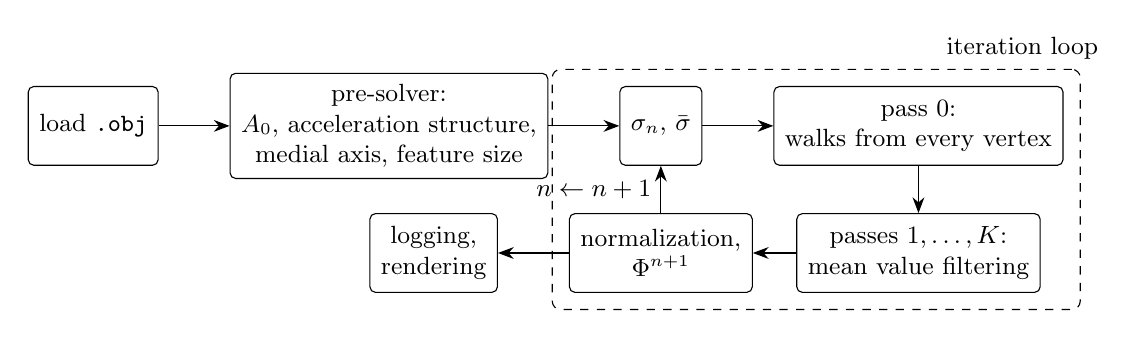
\begin{tikzpicture}[
			node distance=6mm and 9mm,
			box/.style={draw, rounded corners=2pt, align=center, minimum height=10mm, inner sep=4pt, font=\small},
			arr/.style={-{Stealth[length=2mm]}}
			]
			% top row
			\node[box] (obj) {load \texttt{.obj}};
			\node[box, right=of obj] (pre) {pre-solver:\\ $A_0$, acceleration structure,\\ medial axis, feature size};
			\node[box, right=of pre] (sig) {$\sigma_n$, $\bar{\sigma}$};
			\node[box, right=of sig] (p0) {pass 0:\\ walks from every vertex};
			% bottom row
			\node[box, below=of p0] (filt) {passes $1,\dots,K$:\\ mean value filtering};
			\node[box, below=of sig] (norm) {normalization,\\ $\Phi^{n+1}$};
			\node[box, left=of norm] (log) {logging,\\ rendering};
			
			\draw[arr] (obj) -- (pre);
			\draw[arr] (pre) -- (sig);
			\draw[arr] (sig) -- (p0);
			\draw[arr] (p0) -- (filt);
			\draw[arr] (filt) -- (norm);
			\draw[arr] (norm) -- node[left, font=\small] {$n \leftarrow n+1$} (sig);
			\draw[arr] (norm) -- (log);
			
			\node[draw, dashed, rounded corners=3pt, inner sep=6pt, fit=(sig) (p0) (filt) (norm),
			label={[font=\small]above right:iteration loop}] {};
		\end{tikzpicture}
		\caption{Architecture of the solver.}
		\label{fig:architecture}
	\end{figure}
	
	\section{Data structure}
	
	The input surface is a triangle mesh, stored as a list of vertices and a list of triangles.
	A \texttt{Vertex} holds one \texttt{Vector3} (the position), and a \texttt{Triangle} holds three integers \texttt{v0}, \texttt{v1}, \texttt{v2}, the indices of its corners. The program can currently read only \texttt{.obj} files: the loader keeps the \texttt{v} lines as vertices and the \texttt{f} lines as triangles (only the position index of every corner is used), so the input has to be a triangle mesh.
	
	During a walk, the solver has to evaluate functions that are known only at the vertices ($\Phi^n$, $\sigma_n$, the feature size) at arbitrary points of the surface. For this, every surface point is stored as an \texttt{Interp} record, which consists of the indices $v_0, v_1, v_2$ of three vertices and the interpolation weights $w_0, w_1, w_2$ with $w_0 + w_1 + w_2 = 1$.
	
	The function \texttt{closestInterp} asks Mantis for the closest surface point of a query point and converts the answer into an \texttt{Interp}. Mantis reports whether the closest point lies on a vertex, on an edge, or inside a triangle. In the first, case the weight of that vertex is $1$; in the second, the point is interpolated linearly between the two endpoints of the edge; and in the third, the weights are the barycentric coordinates of the point in the triangle. A function $f$ given at the vertices is then evaluated as
	\[
	f(y) \approx w_0 f(v_0) + w_1 f(v_1) + w_2 f(v_2),
	\]
	which is done by \texttt{interpScalar} for scalars and by \texttt{interpVec} for vectors.
	
	The parameters of the solver can be set from the command line; they are listed in Table~\ref{tab:params}.
	
	\begin{table}[ht]
		\centering
		\begin{tabular}{l l l}
			\hline
			Parameter & Example value & Meaning \\
			\hline
			\texttt{delta} & $5 \cdot 10^{-4}$ & time step $\delta$ of one iteration \\
			\texttt{iters} & $300$ & number of iterations \\
			\texttt{Ns} & $30000$ & number of samples of the medial axis point cloud \\
			\texttt{lfsMin} & $0.01$ & lower bound of the feature size (ball radius) \\
			\texttt{Np} & $50$ & walks per vertex in the first pass \\
			\texttt{K} & $3$ & number of filter passes \\
			\texttt{Nw} & $50$ & filtered estimates per vertex in one filter pass \\
			\texttt{Nv} & $5$ & ball samples of one filtered estimate \\
			\texttt{maxSteps} & $4096$ & step limit of one walk \\
			\hline
		\end{tabular}
		\caption{Parameters of the solver.}
		\label{tab:params}
	\end{table}
	
	\section{Pre-solver calculations}
	
	Before starting the iteration loop, the solver does some pre-calculations. The first one is the vertex area $A_0(x_i)$ of the original surface. The function \texttt{vertexAreas} gives every vertex one third of the area of each triangle it belongs to, so the areas of the vertices add up to the area of the surface. The total area $A_{\mathrm{target}} = \sum_i A_0(x_i)$  is saved, because the normalization at the end of every iteration rescales the shape back to it.
	\texttt{vertexAreas} gives every vertex one third of the area of each triangle it belongs to, so the areas of the vertices add up to the area of the surface. The total area (\texttt{targetArea}) is saved, because the normalization at the end of every iteration rescales the shape back to it.
	
	Everything else that depends on the geometry is built by \texttt{rebuildBase}:
	\begin{enumerate}
		\item \textbf{Acceleration structure.} The vertices and triangles are handed to mantis, which builds the structure used by every closest-point query.
		\item \textbf{Medial axis point cloud.} \texttt{Ns} points are sampled, and from them a point cloud $\mathcal{M}$ that approximates the medial axis of the surface is computed.
		\item \textbf{Local feature size.} The radius of the ball a walk may use at vertex $x_i$ is
		\[
		R_i = \max\bigl(0.9 \cdot \min_{m \in \mathcal{M}} \lVert m - x_i \rVert,\ \texttt{lfsMin}\bigr).
		\]
		The factor $0.9$ keeps the ball away from the medial axis, so the closest-point projection of its points is well-defined, the lower bound keeps the walks from stalling where the surface is very thin.
		\item \textbf{Initial state.} $A_0$ is stored and the embedding is initialized as $\Phi^0 = $ the original vertex positions.
	\end{enumerate}
	All of this is computed only once. The walks always live on the original surface $S_0$, which never changes; an iteration only changes the embedding $\Phi^n$, which is stored as one \texttt{Vector3} per vertex.
	
	\section{Iteration loop}

	One iteration computes $\Phi^{n+1}$ from $\Phi^{n}$. It consists of $K+1$ passes over the vertices: pass $0$ estimates the solution with walks, and passes $1, \dots, K$ refine it with mean value filtering. The state of the loop is the iteration index, the pass index, and the index of the next vertex (Algorithm~\ref{alg:iteration}).
	
	\begin{algorithm}[H]
		\small
		\caption[One iteration]{One iteration of the solver: computing $\Phi^{n+1}$ from $\Phi^n$.}
		\label{alg:iteration}
		\begin{algorithmic}[1]
			\Require embedding $\Phi^n$, vertex areas $A_0$ of $S_0$, feature sizes $R_i$, total area $A_{\mathrm{target}}$, time step $\delta$, number of filter passes $K$
			\Ensure embedding $\Phi^{n+1}$
			\State $A_n \gets \textsc{VertexAreas}(\Phi^n)$
			\State $\sigma_n(x_i) \gets A_n(x_i) \,/\, \bigl(\max(A_0(x_i), 10^{-12})\,\delta\bigr)$ for every vertex $x_i$
			\State $\bar\sigma \gets \max_i \sigma_n(x_i)$
			\For{every vertex $x_i$} \Comment{pass $0$: walks}
			\State $u_0(x_i) \gets$ average of $N_p$ walks (Algorithms~\ref{alg:walk} and~\ref{alg:pair})
			\EndFor
			\For{$k = 1, \dots, K$} \Comment{filter passes}
			\For{every vertex $x_i$}
			\State $u_k(x_i) \gets$ average of $N_w$ filtered estimates (Algorithm~\ref{alg:filtered})
			\EndFor
			\EndFor
			\State $\Phi^{n+1} \gets \textsc{Normalize}(u_K, A_{\mathrm{target}})$ \Comment{Section~\ref{sec:normalization}}
		\end{algorithmic}
	\end{algorithm}
	Because the state is kept between frames, the solver does not have to finish a pass in one go. In the windowed mode, it works for at most $0.05$ seconds per frame (\texttt{sliceSec}) and then the current shape is drawn, so the window stays responsive. In the headless mode, there is no time limit, and nothing is drawn. When a pass is finished, \texttt{uPrev} and \texttt{uNew} are swapped, so the next pass can read the result of the previous one.
	
	\subsection{Sigma}
	
	At the start of every iteration, the screening coefficient is computed for every vertex:
	\[
	\sigma_n(x_i) = \frac{1}{\delta} \cdot \frac{A_n(x_i)}{A_0(x_i)},
	\]
	where $A_n$ is the vertex area of the current shape $\Phi^n$ and $A_0$ is the vertex area of $S_0$. The ratio of the two areas is the discrete version of the area distortion between the two metrics.
	In the implementation, $A_0(x_i)$ is bounded from below by $10^{-12}$ to avoid a division by zero.
	Since $\sigma_n$ is not constant, the walks use delta tracking \cite{sawhneyseyb22gridfree} with the constant majorant
	\[
	\bar{\sigma} = \max_i \sigma_n(x_i).
	\]
	
	\subsection{First pass}
	
	In the first pass, \texttt{EstimateSolution} starts \texttt{Np} walks from every vertex $x_i$ and averages their results. One walk (\texttt{WalkEstimate}) repeats the following step from its current point $x$:
	\begin{enumerate}
		\item The radius of the ball is the interpolated feature size $R$ at $x$, and $\kappa = R \sqrt{\bar{\sigma}}$.
		\item With probability $\kappa / \sinh \kappa$, there is \textbf{no collision} inside the ball: a uniformly distributed point is sampled on the sphere of radius $R$, it is projected to its closest point on $S_0$, and the walk continues from there.
		\item Otherwise there is a \textbf{collision} inside the ball. A point $y$ is sampled in the ball with the density of the screened Green's function, and it is projected to $S_0$. With probability $\sigma_n(y) / \bar{\sigma}$ the collision is real: the walk ends and returns $\Phi^n(y)$. Otherwise it is a null collision, and the walk continues from $y$.
	\end{enumerate}
	The whole walk is summarized in Algorithm~\ref{alg:walk}.
	
	\begin{algorithm}[ht]
		\small
		\caption[One walk]{One walk $\textsc{WalkEstimate}(x)$ started from the vertex $x$.}
		\label{alg:walk}
		\begin{algorithmic}[1]
			\Require start point $x \in S$, $\Phi^n$, $\sigma_n$, $\bar\sigma$, feature size $R(\cdot)$, step limit \texttt{maxSteps}
			\Ensure one sample of $\Phi^{n+1}(x)$
			\For{$s = 1, \dots, \texttt{maxSteps}$}
			\State $R \gets$ interpolated feature size at $x$, \quad $\kappa \gets R\sqrt{\bar\sigma}$
			\If{$\mathcal{U}(0,1) < \kappa / \sinh\kappa$} \Comment{no collision}
			\State $y \gets$ uniform random point on $\partial B_R(x)$
			\State $x \gets \operatorname{cp}_S(y)$
			\Else \Comment{collision inside the ball}
			\State $y \gets$ random point in $B_R(x)$ with density $p_G$
			\State $\hat y \gets \operatorname{cp}_S(y)$
			\If{$\mathcal{U}(0,1) < \sigma_n(\hat y) / \bar\sigma$} \Comment{real collision}
			\State \Return $\Phi^n(\hat y)$
			\EndIf
			\State $x \gets \hat y$ \Comment{null collision}
			\EndIf
			\EndFor
			\State \Return $\Phi^n(x)$ \Comment{step limit reached}
		\end{algorithmic}
	\end{algorithm}
	The mean of the returned values is the estimate of $\Phi^{n+1}(x_i)$, so the three coordinates are solved together by the same walks. A walk is stopped after \texttt{maxSteps} steps and returns $\Phi^n$ at its current point. This is only a safety net, and the number of such walks is logged.
	
	Two details of the sampling are worth mentioning. The probability $\kappa / \sinh \kappa$ is evaluated in the form
	\[
	\frac{\kappa}{\sinh \kappa} = \frac{2 \kappa e^{-\kappa}}{1 - e^{-2\kappa}},
	\]
	which does not overflow for a large $\kappa$, and for $\kappa < 10^{-4}$ its Taylor polynomial $1 - \kappa^2 / 6$ is used. The point inside the ball has a uniformly distributed direction and the radius $tR$, where the density of $t \in [0, 1]$ is proportional to
	\[
	t \sinh\bigl(\kappa (1 - t)\bigr).
	\]
	$t$ is drawn with rejection sampling. The bound it needs is the maximum of the density, which is attained where $\tanh(\kappa (1 - t)) = \kappa t$; this equation is solved with bisection.
	
	\paragraph{Mirrored walk pairs.} The walks are started in pairs \cite{Hammersley_Morton_1956}. The two walks of a pair use the same random numbers, but every direction sampled by the second one is multiplied by $-1$ (Algorithm~\ref{alg:pair}).
	
	\begin{algorithm}[ht]
		\small
		\caption[Mirrored walk pair]{A mirrored pair of walks started from the vertex $x$.}
		\label{alg:pair}
		\begin{algorithmic}[1]
			\Require start point $x \in S$
			\Ensure sum of two correlated samples of $\Phi^{n+1}(x)$
			\State draw a random seed
			\State $a \gets \textsc{WalkEstimate}(x)$ with a random generator initialized by the seed
			\State $b \gets \textsc{WalkEstimate}(x)$ with a generator initialized by the same seed, where every sampled direction is multiplied by $-1$
			\State \Return $a + b$
		\end{algorithmic}
	\end{algorithm}
	The estimate stays unbiased, because both walks have the right distribution on their own. The part of the error that is linear in the direction, however, has opposite signs in the two walks and cancels in their mean, which reduces the variance of the estimate.
	
	\subsection{Filters}
	
	The result of the first pass is noisy, and making it more accurate with more walks is expensive. Instead, the solver uses the mean value filtering of the projected walk on spheres method \cite{Sugimoto:2024:PWoS}: the estimate of pass $k-1$ is known at every vertex, so a new estimate needs only \emph{one} step of a walk, and the rest of the walk is replaced by the interpolated previous estimate $u_{k-1}$. For the vertex $x_i$ one filtered estimate (\texttt{FilteredEstimate}) is
	\[
	u_k(x_i) \approx c \, u_{k-1}(z) + \frac{1 - c}{N_v} \sum_{j=1}^{N_v} \Bigl[ p_j \, \Phi^n(y_j) + (1 - p_j) \, u_{k-1}(y_j) \Bigr],
	\]
	where $c = \kappa / \sinh \kappa$, $z$ is the projection of a uniform point of the sphere, $y_j$ are the projections of points sampled in the ball, and $p_j = \sigma_n(y_j) / \bar{\sigma}$. The first term is the case without a collision. In the second term, the random decision between a real and a null collision is replaced by its expected value: with weight $p_j$ the walk would end and return $\Phi^n(y_j)$, and with weight $1 - p_j$ it would continue, which is approximated by $u_{k-1}(y_j)$.
	Algorithm~\ref{alg:filtered} summarizes one filtered estimate.
	
	\begin{algorithm}[ht]
		\small
		\caption[Filtered estimate]{One filtered estimate $\textsc{FilteredEstimate}(x)$ of $u_k(x)$.}
		\label{alg:filtered}
		\begin{algorithmic}[1]
			\Require vertex $x$, $\Phi^n$, previous estimate $u_{k-1}$, $\sigma_n$, $\bar\sigma$, feature size $R(\cdot)$, number of ball samples $N_v$
			\Ensure one estimate of $u_k(x)$
			\State $R \gets$ interpolated feature size at $x$, \quad $\kappa \gets R\sqrt{\bar\sigma}$, \quad $c \gets \kappa / \sinh\kappa$
			\State $z \gets \operatorname{cp}_S(\text{uniform random point on } \partial B_R(x))$
			\State $b \gets 0$
			\For{$j = 1, \dots, N_v$}
			\State $y_j \gets \operatorname{cp}_S(\text{random point in } B_R(x) \text{ with density } p_G)$
			\State $p_j \gets \operatorname{clamp}\bigl(\sigma_n(y_j) / \bar\sigma,\, 0,\, 1\bigr)$
			\State $b \gets b + p_j \, \Phi^n(y_j) + (1 - p_j) \, u_{k-1}(y_j)$
			\EndFor
			\State \Return $c \, u_{k-1}(z) + \dfrac{1 - c}{N_v}\, b$
		\end{algorithmic}
	\end{algorithm}
	\texttt{FilteredSolution} averages \texttt{Nw} such estimates per vertex, again in mirrored pairs. One filtered estimate costs $1 + N_v$ closest-point queries, and its cost does not depend on the length of the walks (although the rejection sampling in the ball becomes slower for large $\kappa$), so a filter pass is cheap compared to the first pass. Every pass averages the previous estimate over the neighbourhood of the vertex, which reduces the noise of the first pass. Each filtered estimate is, however, itself a Monte Carlo estimate and adds a smaller amount of new noise.
	
	\subsection{Normalization}
	\label{sec:normalization}
	After the last pass, \texttt{uPrev} holds the estimate of $\Phi^{n+1}$. The flow shrinks the surface, so before the next iteration the shape is normalized by \texttt{normalizeGeometry}: the area-weighted centroid
	\[
	c = \frac{\sum_i A(x_i) \, \Phi(x_i)}{\sum_i A(x_i)}
	\]
	is moved to the origin, and the shape is scaled so that its total area is the area of the original surface again:
	\[
	\Phi(x_i) \leftarrow s \, \bigl(\Phi(x_i) - c\bigr), \qquad s = \sqrt{\frac{A_{\mathrm{target}}}{\sum_i A(x_i)}}.
	\]
	The normalization keeps the scale of the shape fixed, so the same time step $\delta$ has the same meaning in every iteration. Since it is a similarity transformation, it does not change the shape, only the time parametrization of the flow. Only $\Phi$ is replaced; the surface $S_0$, its acceleration structure, and the feature sizes are left untouched, and the next iteration starts with the computation of $\sigma_{n+1}$.
	
	\section{Logging and error metric}
	\label{sec:logging}
	After every iteration, the solver writes one row into \texttt{metrics.csv} and saves the vertex positions of the current shape, from which the flow can be replayed later. The logged quantities are
	\begin{itemize}
		\item the sphericity $\pi^{1/3} (6V)^{2/3} / A$ of the shape, which is $1$ for a sphere and smaller for everything else,
		\item the statistics of $\sigma_n$ (majorant, mean, median, minimum),
		\item the mean number of steps of a walk and the fraction of the walks that reached the step limit,
		\item the number of closest-point queries, the running time and the memory usage of the iteration,
		\item the quality of the mesh: the smallest angle of the triangles and the smallest ratio between the current and the original area of a triangle.
	\end{itemize}
	To measure the error of the Monte Carlo estimate, the same semi-implicit step is also solved deterministically on the mesh,
	\[
	\bigl(\operatorname{diag}(A_n) + \delta L_0\bigr) \, u = \operatorname{diag}(A_n) \, \Phi^n,
	\]
	where $L_0$ is the cotangent stiffness matrix of $S_0$. The system is solved with the conjugate gradient method. This reference is used only for the comparison and is not part of the solver. The logged error is the root mean square distance between the Monte Carlo result and $u$, relative to the bounding box diagonal of the shape and relative to the displacement of the reference step. Note that this is the error of a single step started from the same $\Phi^n$ (a local error); the errors of the previous steps are not included.
	
	
	% =====================================================================
	% 6. RESULTS
	% =====================================================================
	\chapter{Results and numerical analysis}
	\label{ch:results}
	
	We tested the solver on two models, Spot \cite{crane2013robust} and the Stanford Bunny \cite{tuealga_meshes}, and recorded the quantities listed in Section~\ref{sec:logging} to describe its behaviour and its limitations. Unless stated otherwise, the tests use the base parameters in Table~\ref{tab:params_of_base}. Each configuration was run once with a fixed seed, so small differences between runs should be interpreted with care.
	
	\begin{table}[ht]
		\centering
		\begin{tabular}{l l }
			\hline
			Parameter & Base value \\
			\hline
			\texttt{delta} & $5 \cdot 10^{-3}$\\
			\texttt{iters} & $150$\\
			\texttt{Ns} & $30000$  \\
			\texttt{lfsMin (Spot)} & $0.06$  \\
			\texttt{lfsMin (Bunny)} & $0.055$  \\
			\texttt{Np} & $20$ \\
			\texttt{K} & $5$ \\
			\texttt{Nw} & $50$  \\
			\texttt{Nv} & $1$ \\
			\texttt{maxSteps} & $4096$ \\
			\texttt{seed} & $123$ \\
			\hline
		\end{tabular}
		\caption{Base parameters of the tests.}
		\label{tab:params_of_base}
	\end{table}
	
	\begin{remark}
		We only varied the time step $\delta$, the number of filter passes $K$ and \texttt{lfsMin}. In preliminary experiments, changing the other parameters did not affect the measured quantities notably.
	\end{remark}
	All measurements were made with an AMD Ryzen 5 7530U CPU with 16 GB of RAM.
	
	\section{Convergence}
	\label{convergance}
	
	Figure~\ref{fig:sphericity_delta} shows how the sphericity changes during the flow for different values of $\delta$. Note that the horizontal axis is the number of iterations; one iteration advances the flow by $\delta$, so a larger $\delta$ is expected to converge in fewer iterations.
	
	\begin{figure}[H]
		\centering
		\begin{subfigure}{0.49\textwidth}
			\centering
			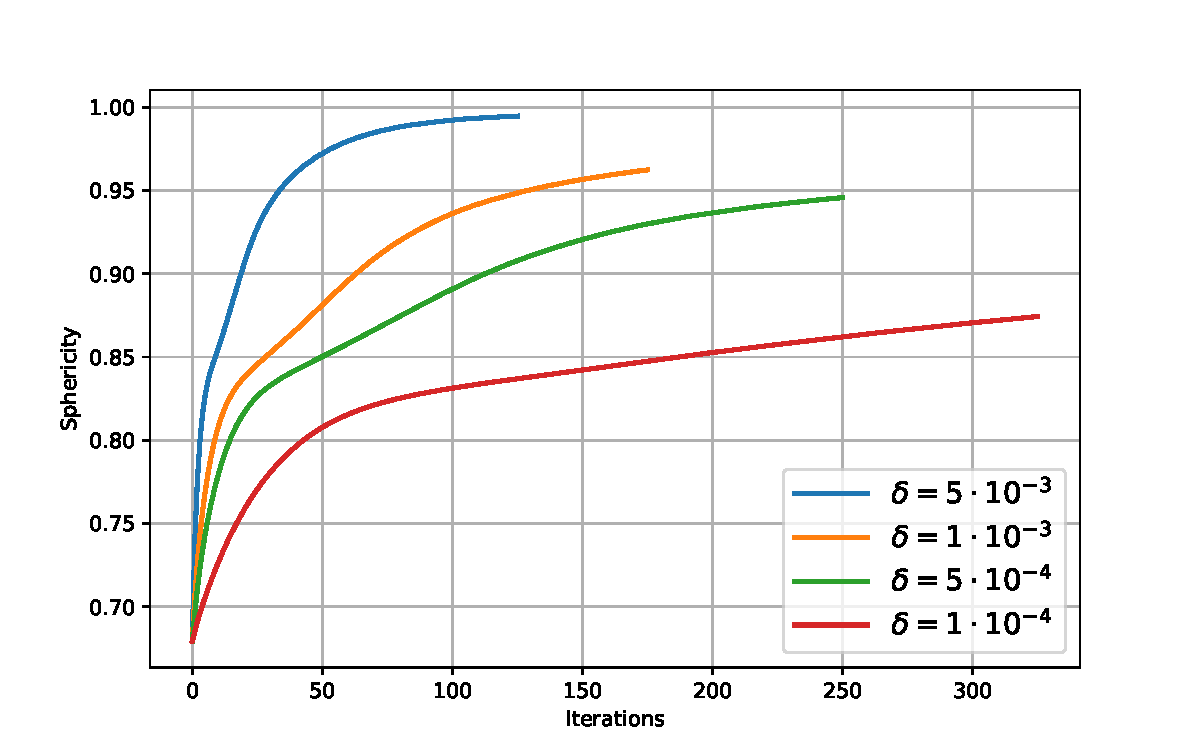
\includegraphics[width=\linewidth]{images/spot_base_delta_spher.pdf}
			\caption{Spot}
			\label{fig:deltaOnBaseSpotSpher}
		\end{subfigure}
		\hspace{0.00\textwidth}
		\begin{subfigure}{0.49\textwidth}
			\centering
			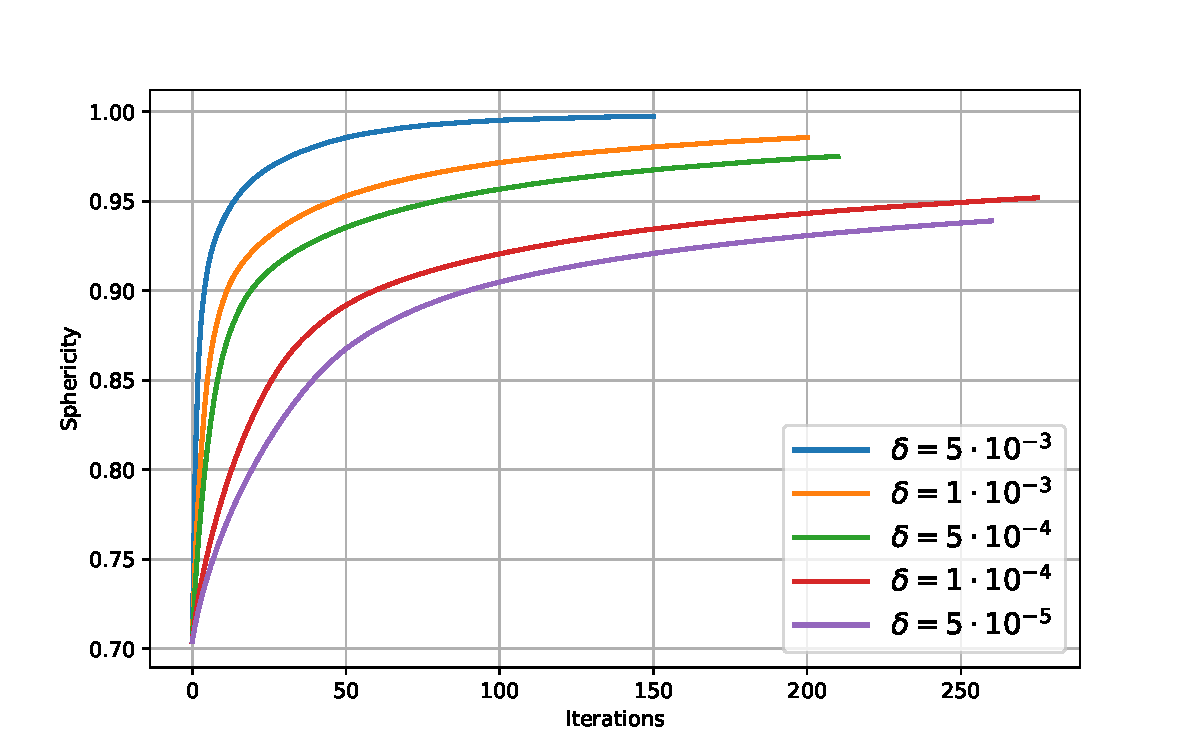
\includegraphics[width=\linewidth]{images/bunny_base_delta_spher.pdf}
			\caption{Bunny}
			\label{fig:deltaOnBaseBunnySpher}
		\end{subfigure}
		\caption{How $\delta$ affects the sphericity on Spot and the Bunny}
		\label{fig:sphericity_delta}
	\end{figure}
	The time step $\delta$ has a large effect on the convergence. With a larger $\delta$, the surface approaches the sphere in fewer iterations, but, as shown in Sections~\ref{error} and~\ref{meshHealt}, each step has a larger error, and the mesh degrades more. With a smaller $\delta$, the error of a single step is smaller, but many more iterations are needed; the total running time is much longer (Section~\ref{wpsNtpw}), and, as shown in Section~\ref{error}, the accumulated error at the same flow time is actually larger.
	
	\begin{figure}[H]
		\centering
		\begin{subfigure}{0.2\textwidth}
			\centering
			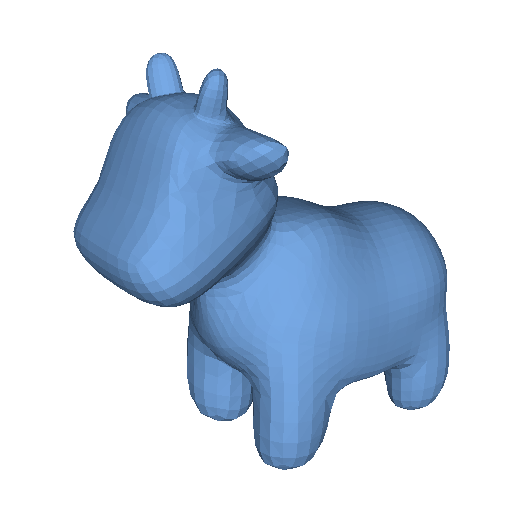
\includegraphics[width=\linewidth]{images/spot_base_iter_0.png}
			\caption{Iteration 0}
		\end{subfigure}
		\hspace{0.05\textwidth}
		\begin{subfigure}{0.2\textwidth}
			\centering
			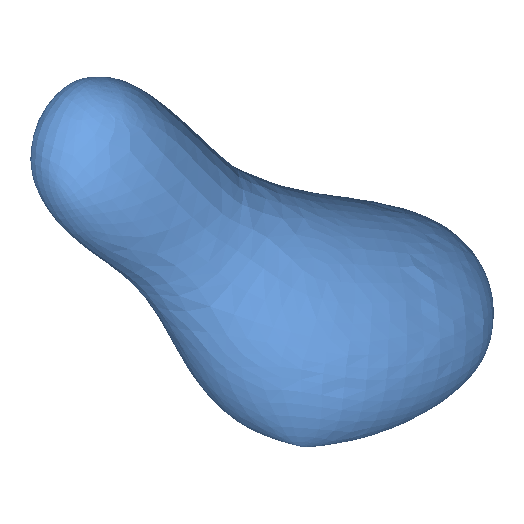
\includegraphics[width=\linewidth]{images/spot_base_iter_10.png}
			\caption{Iteration 10}
		\end{subfigure}
		
		\vspace{1em}
		
		\begin{subfigure}{0.2\textwidth}
			\centering
			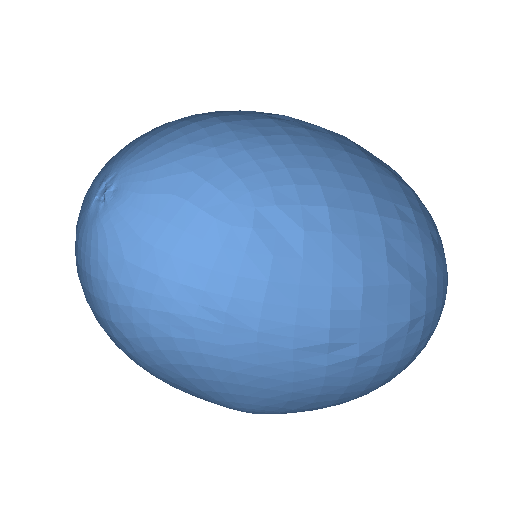
\includegraphics[width=\linewidth]{images/spot_base_iter_50.png}
			\caption{Iteration 50}
		\end{subfigure}
		\hspace{0.05\textwidth}
		\begin{subfigure}{0.2\textwidth}
			\centering
			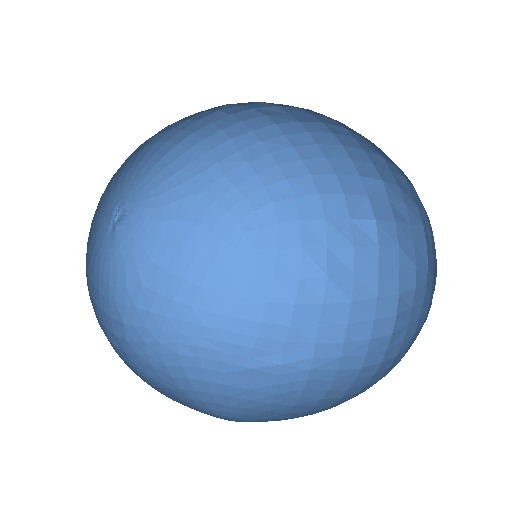
\includegraphics[width=\linewidth]{images/spot_base_iter_125.png}
			\caption{Iteration 125}
		\end{subfigure}
		
		\caption{Spot during the flow with $\delta = 5 \cdot 10^{-3}$}
		\label{fig:deltaOnBaseSpotSphere}
	\end{figure}
	
	Changing \texttt{lfsMin} or the number of filter passes has almost no effect on the rate of convergence or on the final sphericity (Table~\ref{tab:time_of_tests}).
	
	\section{Error analysis}
	\label{error}
	The error is measured as described in Section~\ref{sec:logging}: in every iteration, the Monte Carlo result is compared to the deterministic solution of the same step, started from the same $\Phi^n$. It is therefore the error of a single step. Since a smaller $\delta$ needs more steps to reach the same flow time, these per-step errors cannot be compared directly across different values of $\delta$.
	\begin{figure}[H]
		\centering
		\begin{subfigure}{0.49\textwidth}
			\centering
			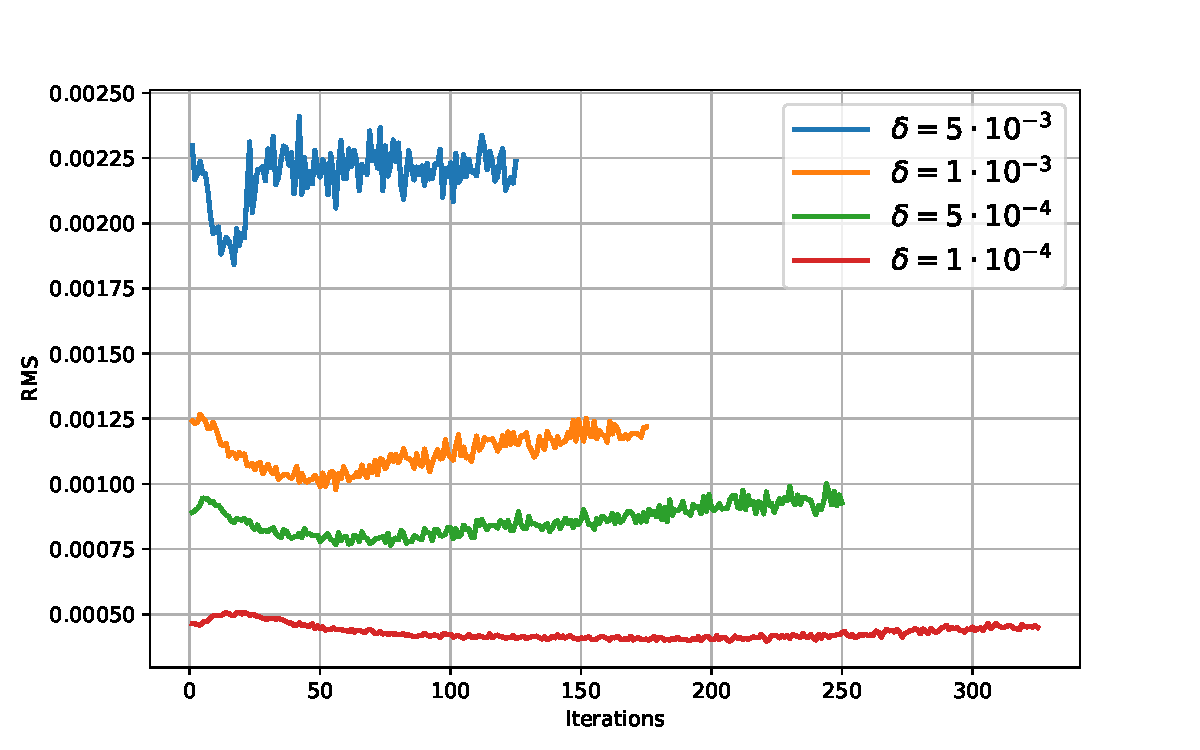
\includegraphics[width=\linewidth]{images/spot_base_delta_error.pdf}
			\caption{Spot}
			\label{fig:deltaOnBaseSpotError}
		\end{subfigure}
		\hspace{0.00\textwidth}
		\begin{subfigure}{0.49\textwidth}
			\centering
			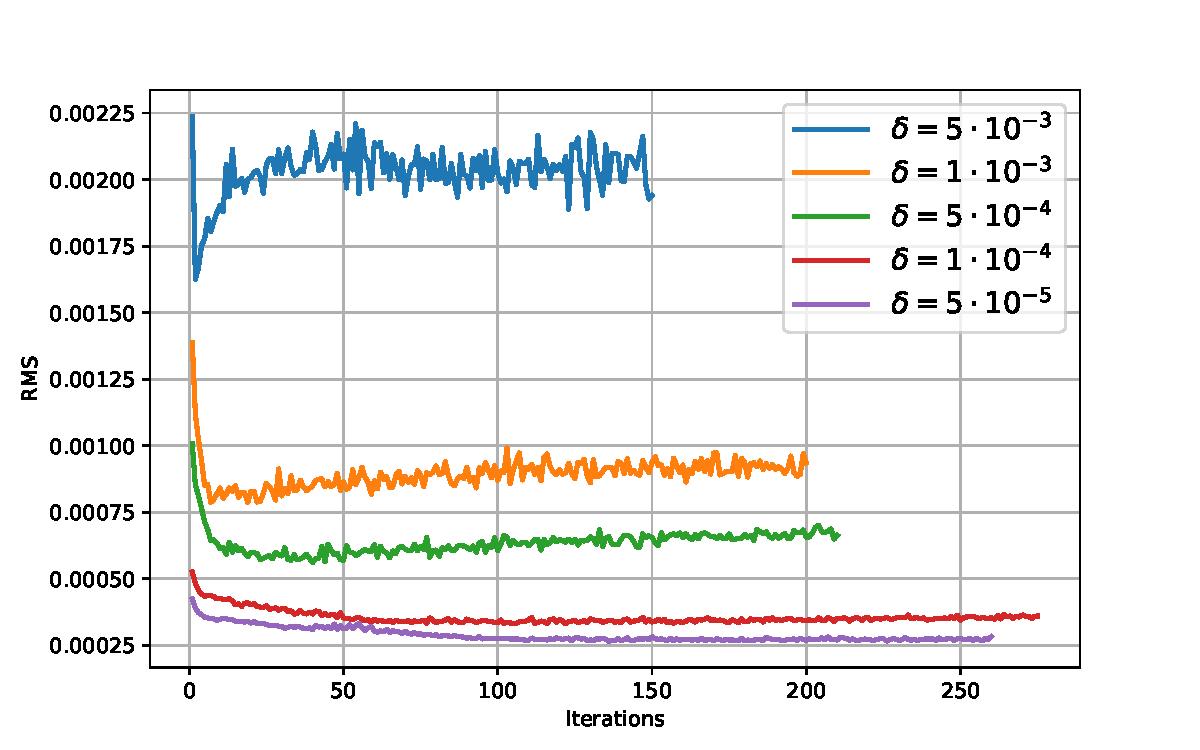
\includegraphics[width=\linewidth]{images/bunny_base_delta_error.pdf}
			\caption{Bunny}
			\label{fig:deltaOnBaseBunnyError}
		\end{subfigure}
		\caption{Effect of $\delta$ on the per-step error on Spot and the Bunny.}
	\end{figure}
	
	\begin{figure}[H]
		\centering
		\begin{subfigure}{0.49\textwidth}
		\centering
			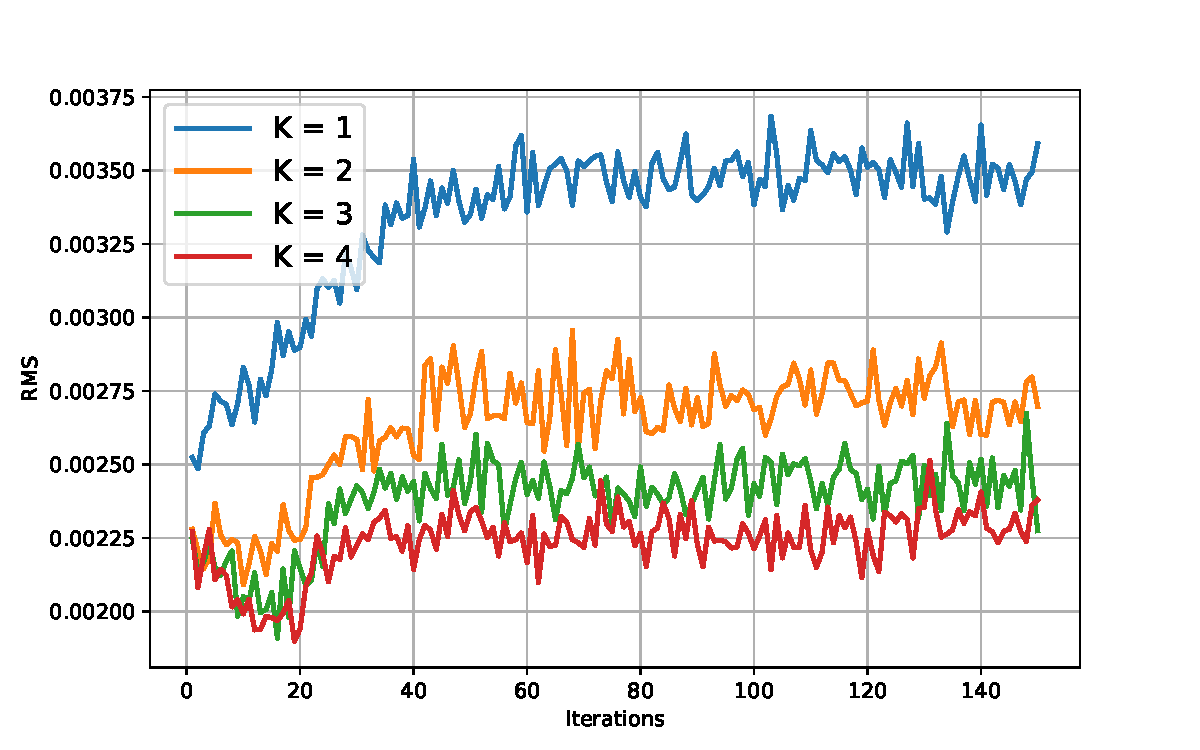
\includegraphics[width=\linewidth]{images/spot_base_K_error.pdf}
			\caption{Effect of different numbers of filters}
			\label{fig:KOnBaseSpotError}
		\end{subfigure}
		\begin{subfigure}{0.49\textwidth}
			\centering
			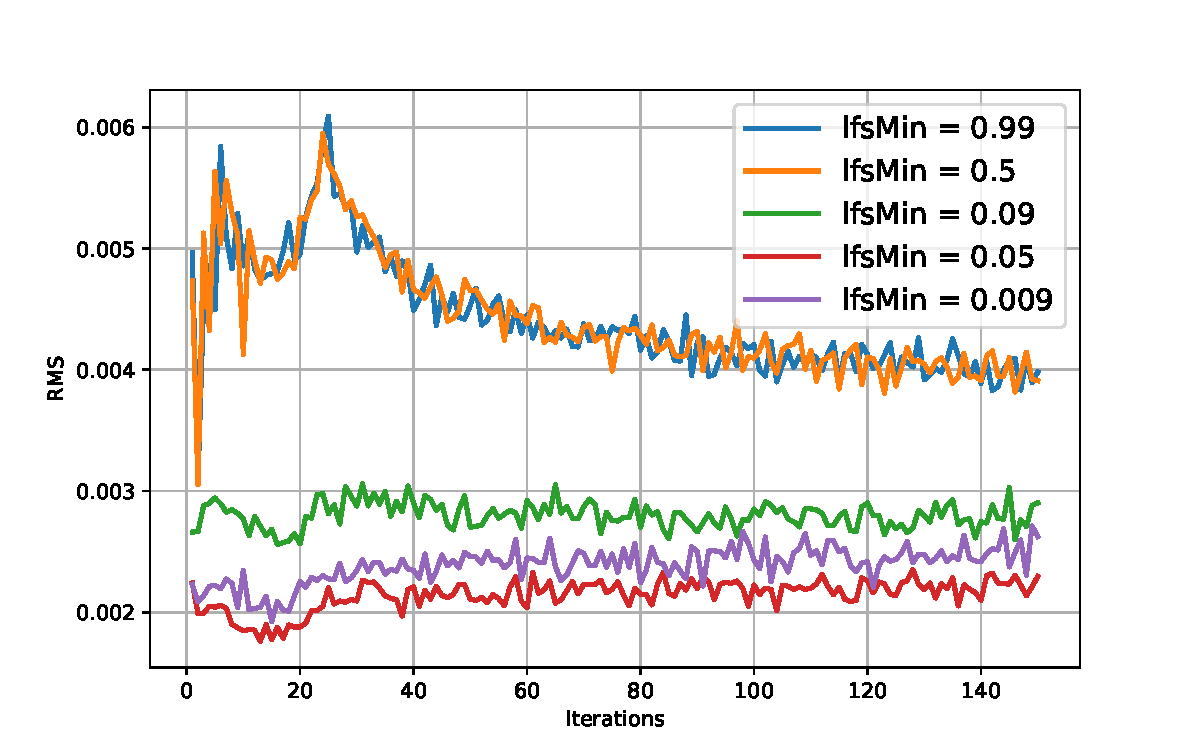
\includegraphics[width=\linewidth]{images/spot_base_lfs_error.pdf}
			\caption{Effect of different values of lfsMin}
			\label{fig:lfsOnBaseSpotError}
		\end{subfigure}
		\caption{Effect of the number of filter passes $K$ and of \texttt{lfsMin} on the per-step error on Spot.}
	\end{figure}
	The per-step error depends strongly on $\delta$. More filter passes also reduce the error, but their effect is smaller than that of $\delta$. The choice of \texttt{lfsMin} matters as well: both too small ($\texttt{lfsMin} \le 0.009$) and too large ($\texttt{lfsMin} \ge 0.09$) values increase the error. On Spot, the lowest error was observed around $\texttt{lfsMin} \approx 0.05$.
	
	\paragraph{Accumulated error.} To measure the accumulated error, we replayed every run with the deterministic step from the initial surface, using the same sequence of time steps, and compared the two flows at every iteration. Table~\ref{tab:global_delta} compares the time steps at the same flow time $t = n\delta$. Although a smaller $\delta$ has a smaller per-step error, its accumulated error is larger because it needs more steps to reach the same flow time, and every step adds noise.
	
	\begin{table}[H]
		\centering
		\begin{tabular}{l c c c c}
			\hline
			& \multicolumn{2}{c}{Spot} & \multicolumn{2}{c}{Bunny} \\
			$\delta$ & $t = 0.013$ & $t = 0.1$ & $t = 0.013$ & $t = 0.1$ \\
			\hline
			$5\cdot10^{-3}$ & 0.69\%$^*$ & 2.26\% & 0.64\%$^*$ & 1.02\% \\
			$1\cdot10^{-3}$ & 1.31\% & 4.64\% & 1.23\% & 1.32\% \\
			$5\cdot10^{-4}$ & 1.92\% & 5.39\% & 1.18\% & 1.39\% \\
			$1\cdot10^{-4}$ & 6.18\% & --     & 2.58\% & --     \\
			$5\cdot10^{-5}$ & --     & --     & 3.67\% & --     \\
			\hline
		\end{tabular}
		\caption{Accumulated error at the same flow time: RMS distance between the Monte Carlo and the deterministic flow, relative to the bounding box diagonal. $^*$At $t = 0.015$ (iteration 3). A dash means that the run did not reach this flow time.}
		\label{tab:global_delta}
	\end{table}
	
	\section{Walk steps and time}
	\label{wpsNtpw}
	
	An iteration consists of two parts: the first pass, which runs PWoS walks with few samples, and the $K$ filter passes. Their costs behave differently, so we discuss them separately. Figures~\ref{fig:stp_tpw_base_spot} and~\ref{fig:stp_tpw_base_bunny} show that for small values of $\delta$ the time per iteration closely follows the number of steps per walk, i.e.\ the first pass dominates the cost.  
	
	\begin{figure}[H]
		\centering
		\begin{subfigure}{0.49\textwidth}
			\centering
			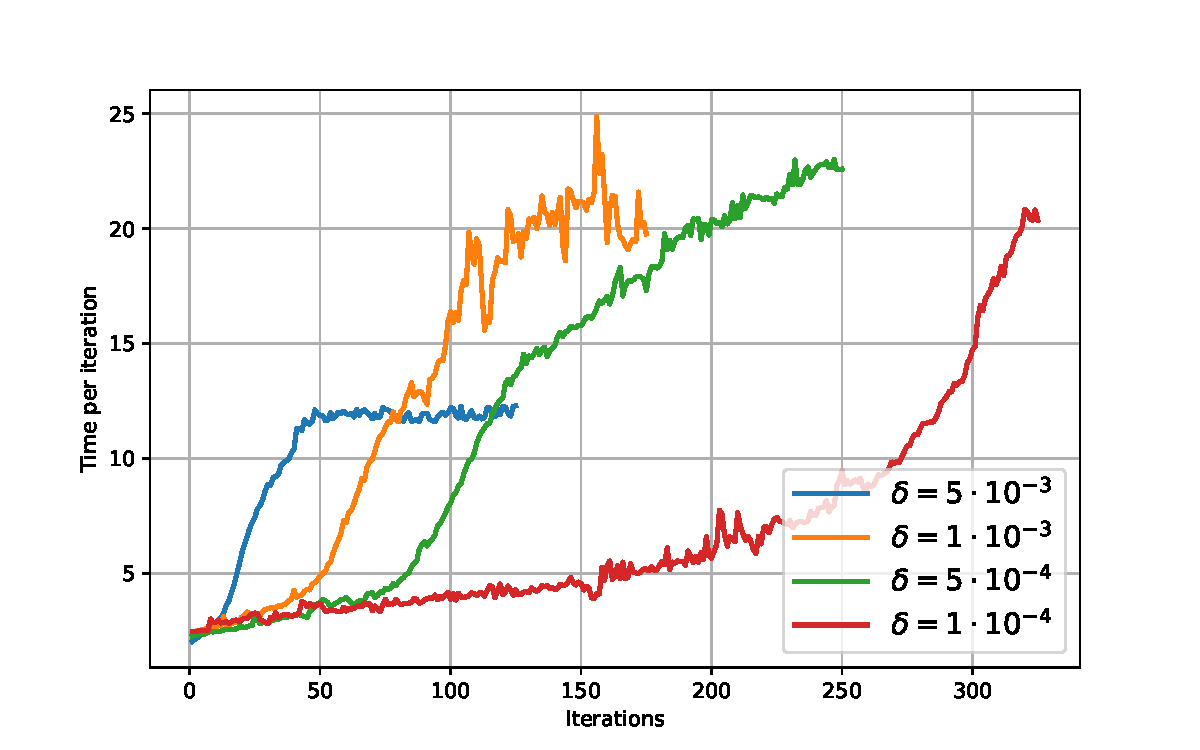
\includegraphics[width=\linewidth]{images/spot_base_delta_tpi.pdf}
			\caption{Time per iteration}
		\end{subfigure}
		\hspace{0.00\textwidth}
		\begin{subfigure}{0.49\textwidth}
			\centering
			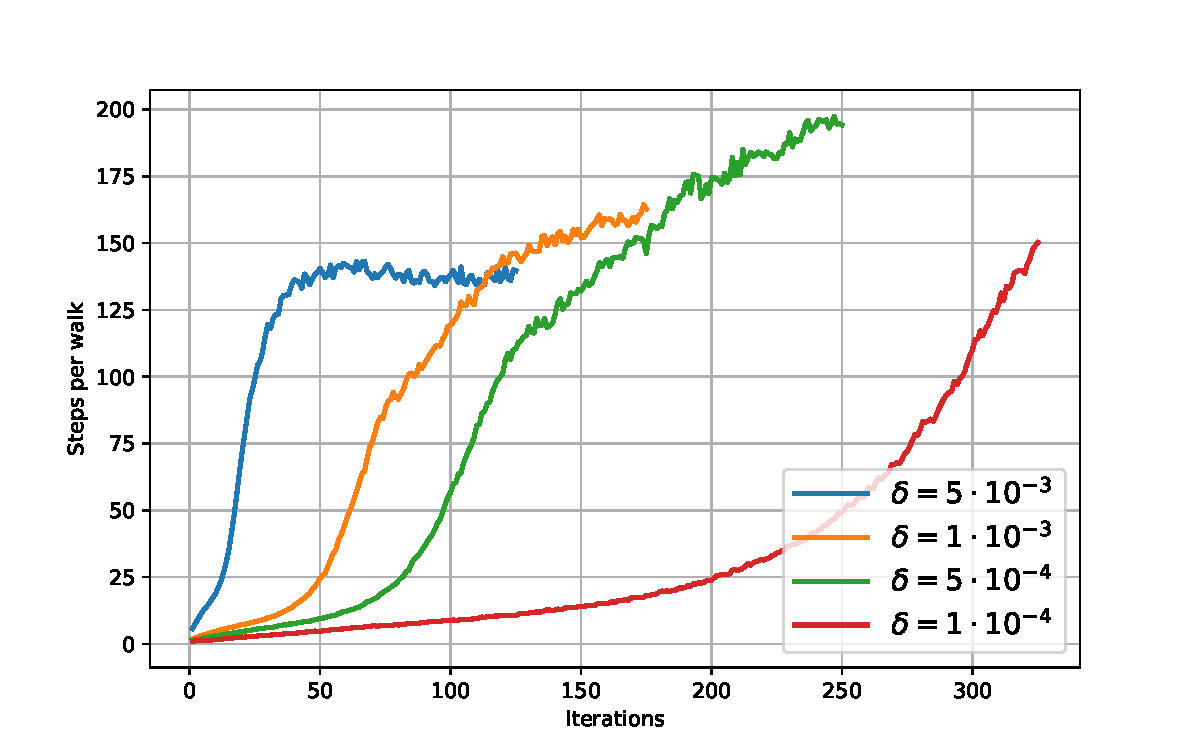
\includegraphics[width=\linewidth]{images/spot_base_delta_spw.pdf}
			\caption{Steps per walk}
		\end{subfigure}
		\caption{Effect of $\delta$ on the time per iteration and the steps per walk on Spot.}
		\label{fig:stp_tpw_base_spot}
	\end{figure}
	
	\begin{figure}[H]
		\centering
		\begin{subfigure}{0.49\textwidth}
			\centering
			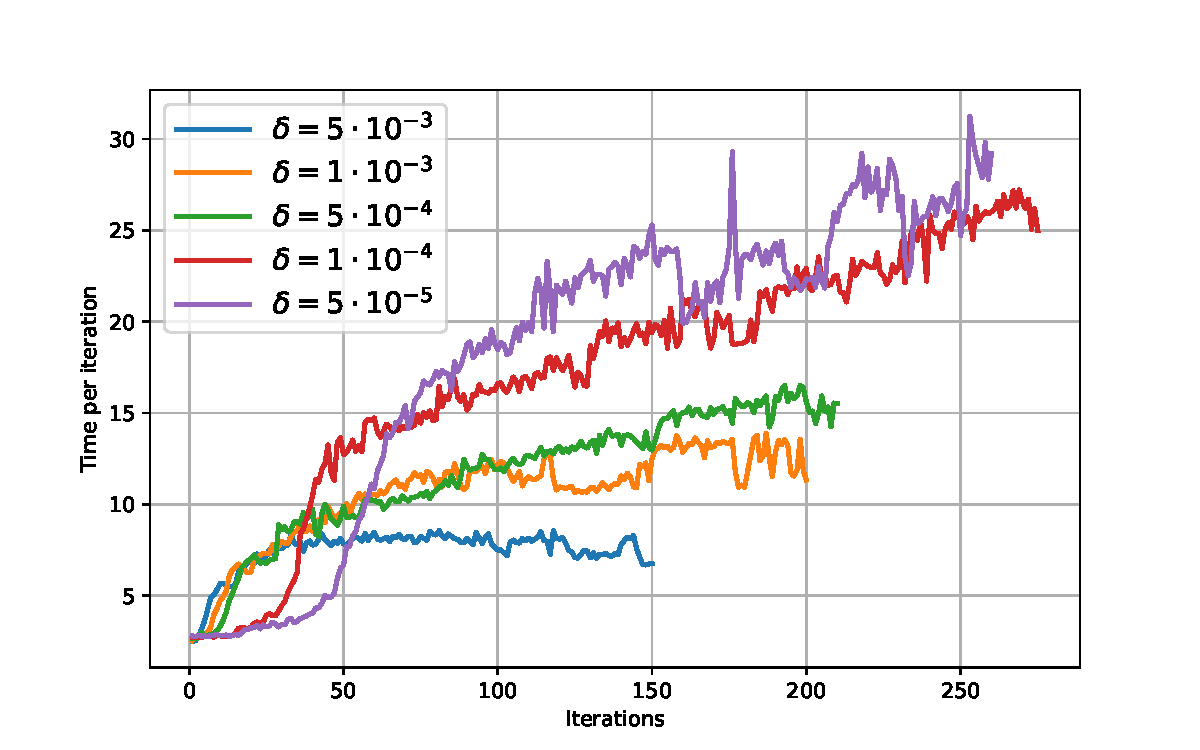
\includegraphics[width=\linewidth]{images/bunny_base_delta_tpi.pdf}
			\caption{Time per iteration}
		\end{subfigure}
		\hspace{0.00\textwidth}
		\begin{subfigure}{0.49\textwidth}
			\centering
			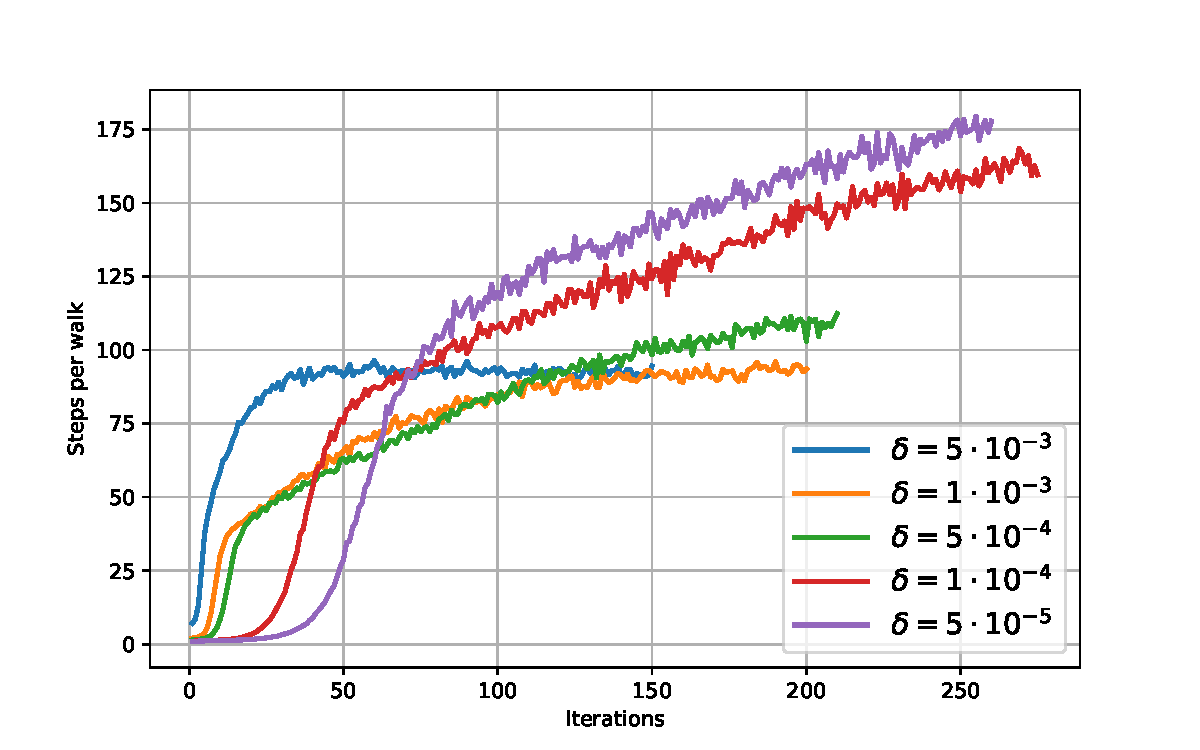
\includegraphics[width=\linewidth]{images/bunny_base_delta_tpw.pdf}
			\caption{Steps per walk}
		\end{subfigure}
		\caption{Effect of $\delta$ on the time per iteration and the steps per walk on the Bunny.}
		\label{fig:stp_tpw_base_bunny}
	\end{figure}
	For the largest value of $\delta$, the filter passes dominate the cost (Figure~\ref{fig:stp_tpw_base_spot_K}). The cost of a filter pass is roughly fixed ($1+N_v$ closest-point queries per estimate), while the length of the walks in the first pass depends on $\delta$ and on the current shape.
	\begin{figure}[H]
		\centering
		\begin{subfigure}{0.49\textwidth}
			\centering
			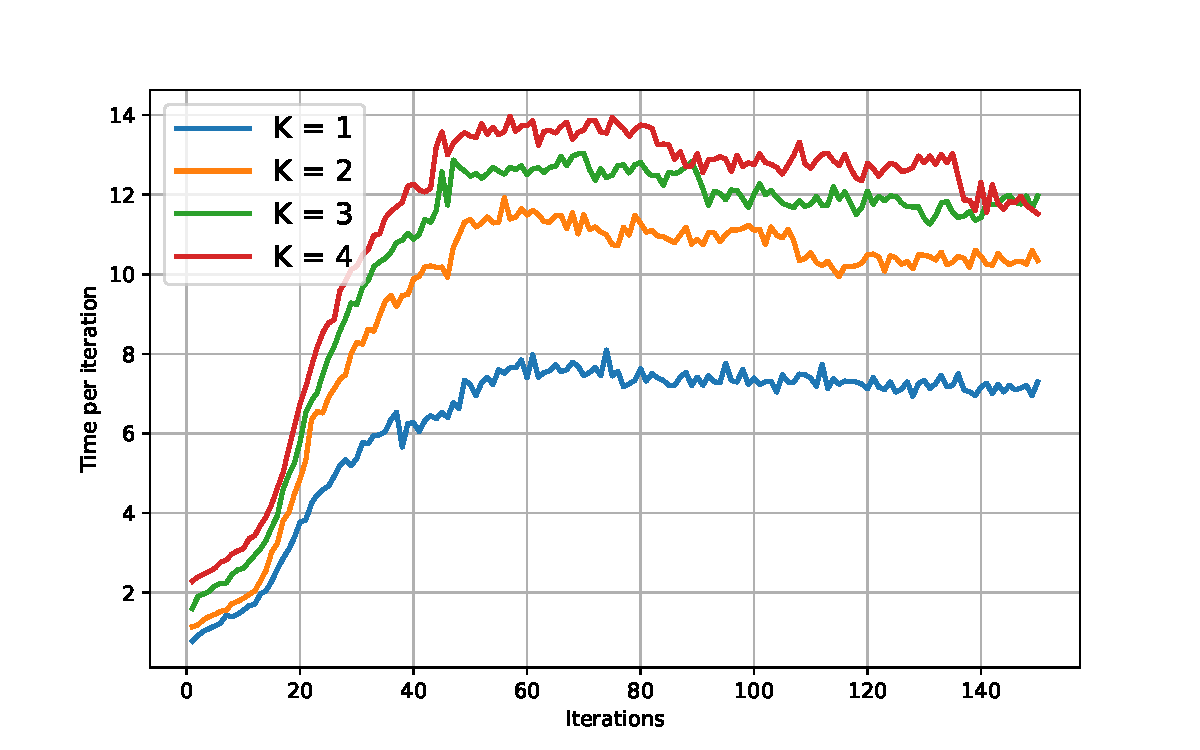
\includegraphics[width=\linewidth]{images/spot_base_K_tpi.pdf}
			\caption{Time per iteration}
		\end{subfigure}
		\hspace{0.00\textwidth}
		\begin{subfigure}{0.49\textwidth}
			\centering
			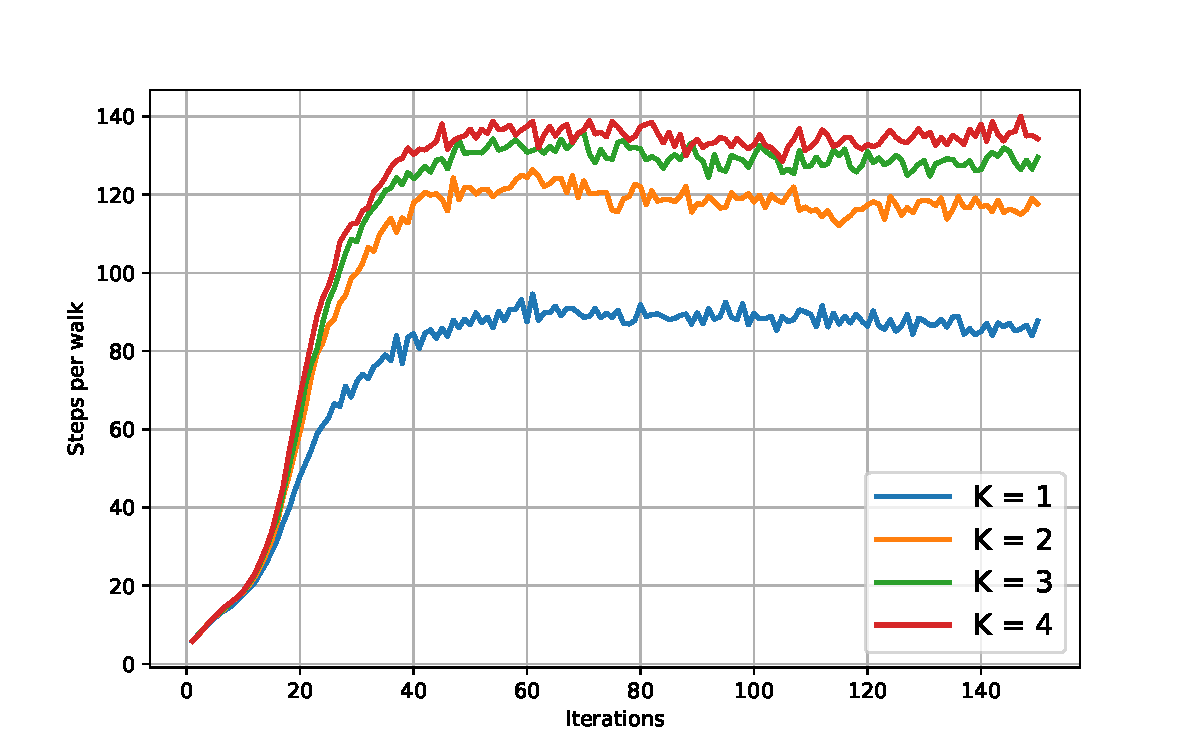
\includegraphics[width=\linewidth]{images/spot_base_K_spw.pdf}
			\caption{Steps per walk}
		\end{subfigure}
		\caption{Effect of the number of filter passes $K$ on the time per iteration and the steps per walk on Spot.}
		\label{fig:stp_tpw_base_spot_K}
	\end{figure}
	Figure~\ref{fig:f} shows that \texttt{lfsMin} also affects the length of the walks: a larger lower bound gives larger balls in thin regions, hence fewer steps per walk and a shorter running time (Table~\ref{tab:time_of_tests}). From the point of view of efficiency, a large \texttt{lfsMin} would therefore be preferable, but it increases the error (Figure~\ref{fig:lfsOnBaseSpotError}) and violates the assumption $B_r(x) \subset \mathcal N(S)$ in more places. We prefer a lower error, since the running time can also be reduced by parallelization. In the tests, we used $\texttt{lfsMin} = 0.06$.
	\begin{figure}[H]
		\centering
		\begin{subfigure}{0.49\textwidth}
			\centering
			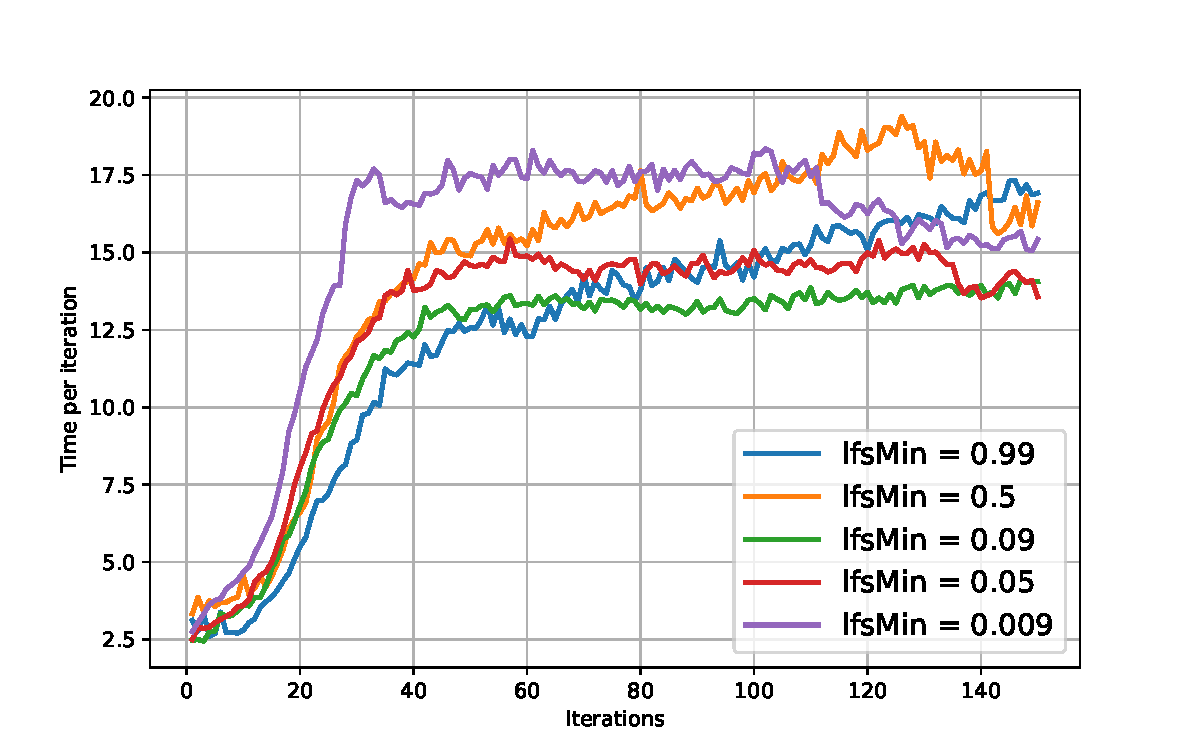
\includegraphics[width=\linewidth]{images/spot_base_lfs_tpi.pdf}
			\caption{Time per iteration}
		\end{subfigure}
		\hspace{0.00\textwidth}
		\begin{subfigure}{0.49\textwidth}
			\centering
			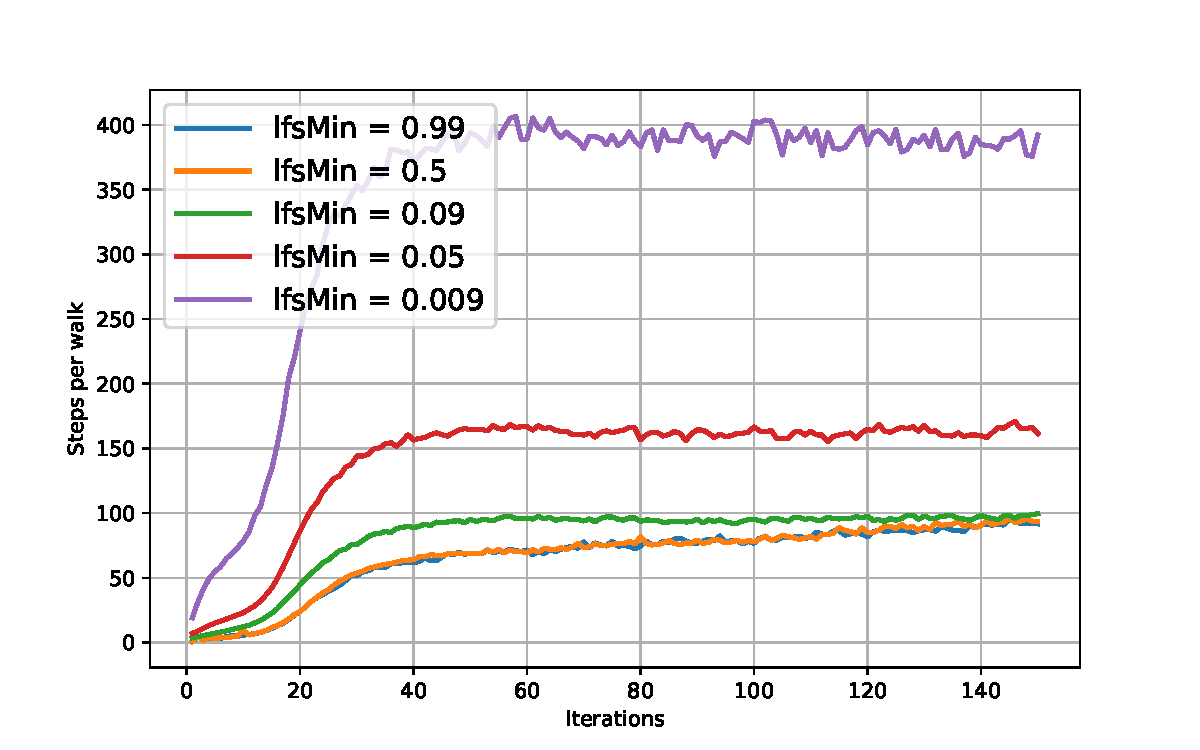
\includegraphics[width=\linewidth]{images/spot_base_lfs_spw.pdf}
			\caption{Steps per walk}
		\end{subfigure}
		\caption{Effect of \texttt{lfsMin} on the time per iteration and the steps per walk on Spot.}
		\label{fig:f}
	\end{figure}
	
	Table~\ref{tab:time_of_tests} summarises the total running time of the tests on Spot.
	
	\begin{table}[H]
		\centering
		\begin{tabular}{l l l l l}
			\hline
			Test & Time & Time (s) & Iterations & Sphericity  \\
			\hline
			$\delta = 5 \cdot 10^{-3}$ & 20 min 48 sec & 1248.1 & 125 & 0.9946 \\
			$\delta = 1 \cdot 10^{-3}$ & 36 min 22 sec & 2182.2 & 175 & 0.9624 \\
			$\delta = 5 \cdot 10^{-4}$ & 50 min 39 sec & 3038.7 & 250 & 0.9458 \\
			$K = 1$ & 15 min 47 sec & 946.8 & 150 & 0.9874 \\
			$K = 4$ & 28 min 21 sec & 1701.0 & 150 & 0.9954 \\
			\texttt{lfsMin} $= 0.99$ & 30 min 59 sec & 1859.6 & 150 & 0.9952 \\
			\texttt{lfsMin} $= 0.06$ & 32 min 2 sec & 1922.2 & 150 & 0.9956 \\
			\texttt{lfsMin} $= 0.009$ & 38 min 3 sec & 2283.4 & 150 & 0.9946 \\
			\hline
		\end{tabular}
		\caption{Running time of the tests on Spot.}
		\label{tab:time_of_tests}
	\end{table}
	
	
	\section{Mesh health}
	\label{meshHealt}
	
	We measured the quality of the mesh in two ways: by the angles of the triangles and by the number of flipped triangles, i.e.\ triangles whose normal points inwards. Table~\ref{tab:bad_triangles} shows that the triangles do not keep their angles during the flow, which we attribute mainly to the noise of the Monte Carlo estimates. The minimum angle is determined by a single triangle and is therefore noisy. The median of the per-triangle minimum angles barely changes, and only $0.2$--$2.2\%$ of the triangles become thin, so the damage is local. A smaller $\delta$ produces fewer thin triangles.
	
	\begin{table}[H]
		\centering
		\small
		\begin{tabular}{l c c c c c c c}
			\hline
			Test & $\delta$ & $K$ & lfsMin & Iter. & Min.\ angle ($^\circ$) & Median ($^\circ$) & Thin ($\%$) \\
			\hline
			\multicolumn{8}{c}{\textit{Spot} \quad (original: min.\ $10.21^\circ$, median $39.0^\circ$, thin $0\%$)} \\
			\hline
			$\delta$ & $5\cdot10^{-3}$ & 5 & 0.06  & 125 & 0.46 & 34.5 & 1.62 \\
			& $5\cdot10^{-4}$ & 5 & 0.06  & 250 & 0.73 & 30.8 & 1.30 \\[2pt]
			$K$      & $5\cdot10^{-3}$ & 1 & 0.06  & 150 & 0.80 & 32.0 & 1.66 \\
			& $5\cdot10^{-3}$ & 4 & 0.06  & 150 & 0.73 & 34.6 & 0.87 \\[2pt]
			lfsMin   & $5\cdot10^{-3}$ & 5 & 0.99  & 150 & 0.25 & 34.8 & 1.30 \\
			& $5\cdot10^{-3}$ & 5 & 0.009 & 150 & 0.42 & 34.0 & 2.17 \\
			\hline
			\multicolumn{8}{c}{\textit{Bunny} \quad (original: min.\ $20.71^\circ$, median $56.8^\circ$, thin $0\%$)} \\
			\hline
			$\delta$ & $5\cdot10^{-3}$ & 5 & 0.055 & 150 & 0.17 & 53.8 & 0.56 \\
			& $5\cdot10^{-4}$ & 5 & 0.055 & 210 & 1.06 & 50.7 & 0.53 \\
			& $5\cdot10^{-5}$ & 5 & 0.055 & 260 & 2.26 & 53.0 & 0.24 \\
			\hline
		\end{tabular}
		\caption{Mesh quality at the final state. Min.\ angle: the smallest angle in the mesh. Median: the median of the per-triangle minimum angles. Thin: the percentage of triangles with minimum angle below $5^\circ$.}
		\label{tab:bad_triangles}
	\end{table}
	
	\begin{figure}[H]
		\centering
		\begin{subfigure}{0.45\textwidth}
			\centering
			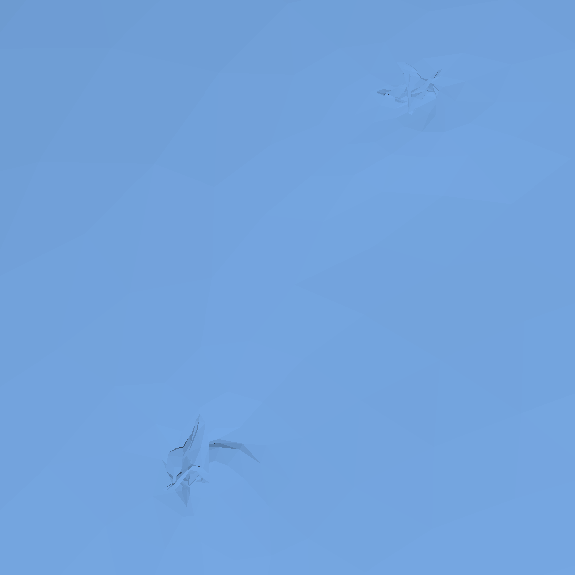
\includegraphics[width=\linewidth]{images/error_on_bunny_ear.png}
			\caption{Base view}
		\end{subfigure}
		\hspace{0.05\textwidth}
		\begin{subfigure}{0.45\textwidth}
			\centering
			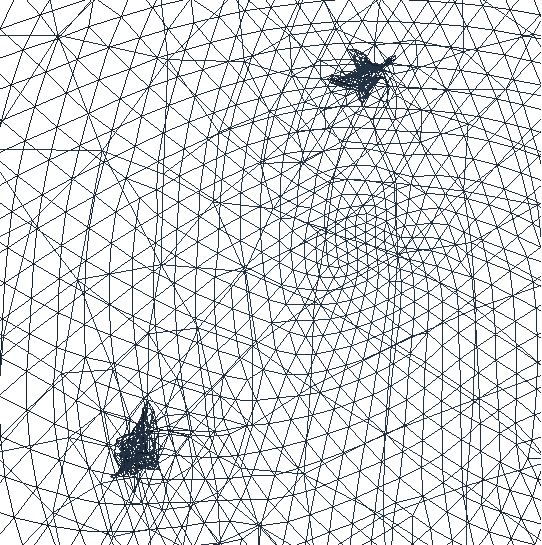
\includegraphics[width=\linewidth]{images/error_on_bunny_ear_wire.png}
			\caption{Mesh/Wire view}
		\end{subfigure}
		\caption{The ears of the Bunny become badly meshed with $\delta = 5 \cdot 10^{-3}$.}
		\label{fig:error_on_ears}
	\end{figure}
	
	The second measure is the percentage of flipped triangles. We classify a triangle as flipped if its normal points towards the centroid of the surface. On a non-convex surface, many triangles are classified as flipped already at the start, so this measure is only meaningful once the surface is nearly spherical (sphericity above about $0.9$). Figure~\ref{fig:flipped_base} shows that the percentage is high at the start and drops quickly as the surface becomes round (Section~\ref{convergance}). Later it rises again, because the noise of the estimates flips some triangles of the already round surface.

	\begin{figure}[H]
		\centering
		\begin{subfigure}{0.49\textwidth}
			\centering
			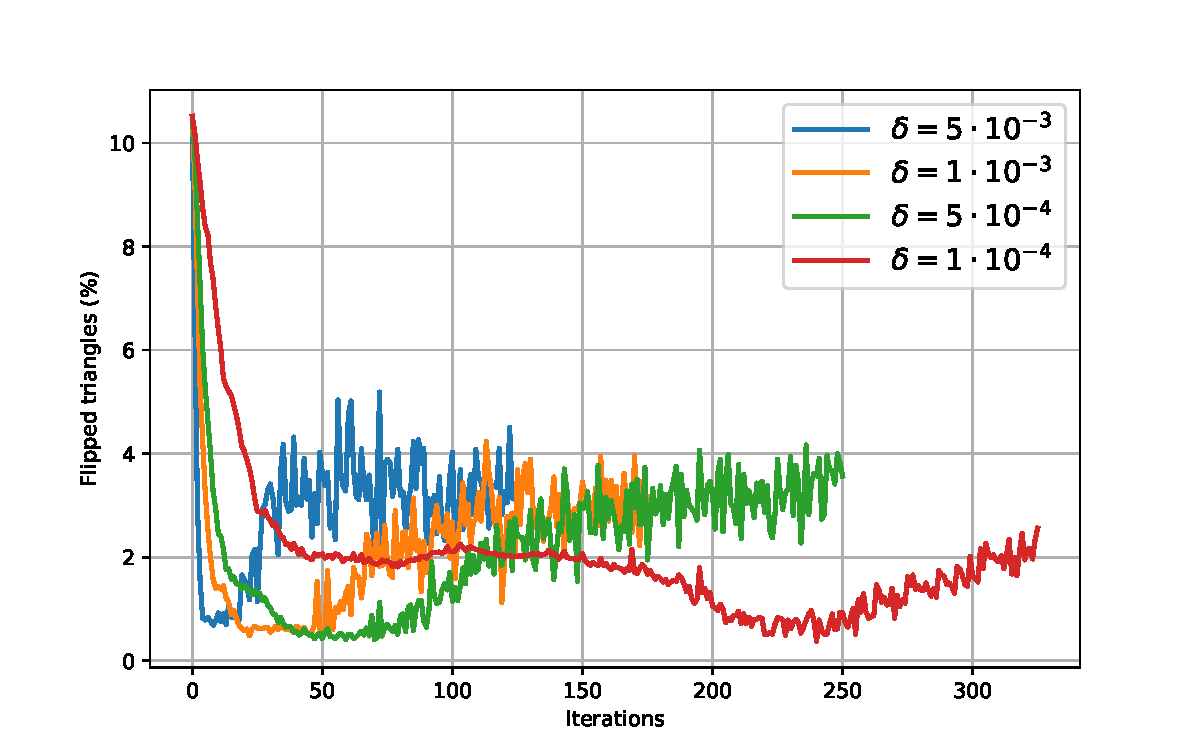
\includegraphics[width=\linewidth]{images/spot_base_delta_flipped.pdf}
			\caption{Effect of $\delta$ on Spot}
			\label{fig:spot_delta_flipped_base}
		\end{subfigure}
		\begin{subfigure}{0.49\textwidth}
			\centering
			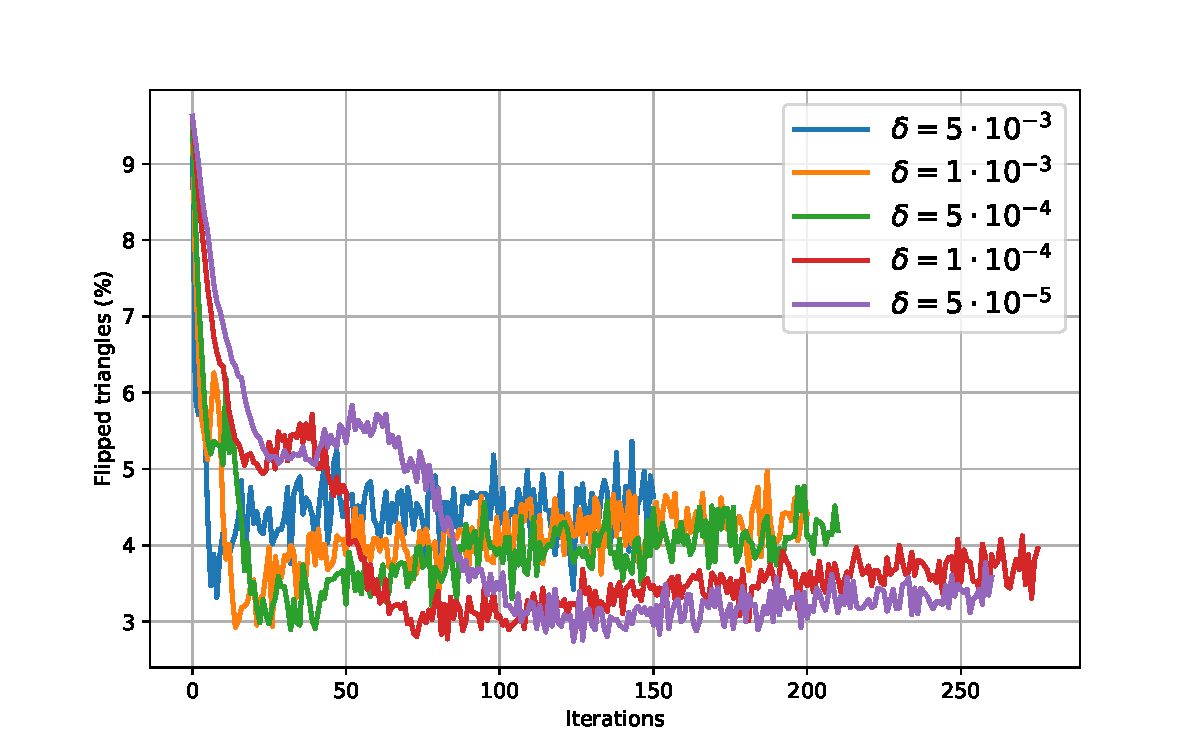
\includegraphics[width=\linewidth]{images/bunny_base_delta_flipped.pdf}
			\caption{Effect of $\delta$ on the Bunny}
			\label{fig:bunny_delta_flipped_base}
		\end{subfigure}
		\vspace{0.5em}
		\begin{subfigure}{0.49\textwidth}
			\centering
			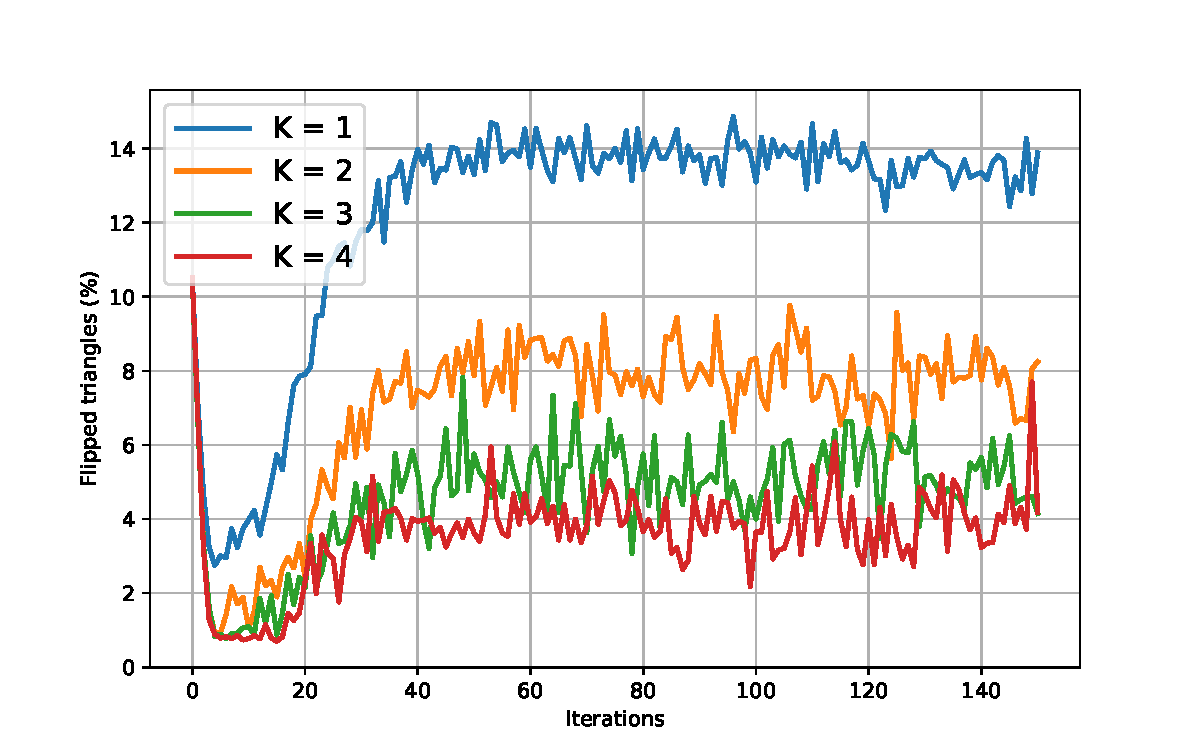
\includegraphics[width=\linewidth]{images/spot_base_K_flipped.pdf}
			\caption{Effect of $K$ on Spot}
			\label{fig:spot_K_flipped_base}
		\end{subfigure}
		\begin{subfigure}{0.49\textwidth}
			\centering
			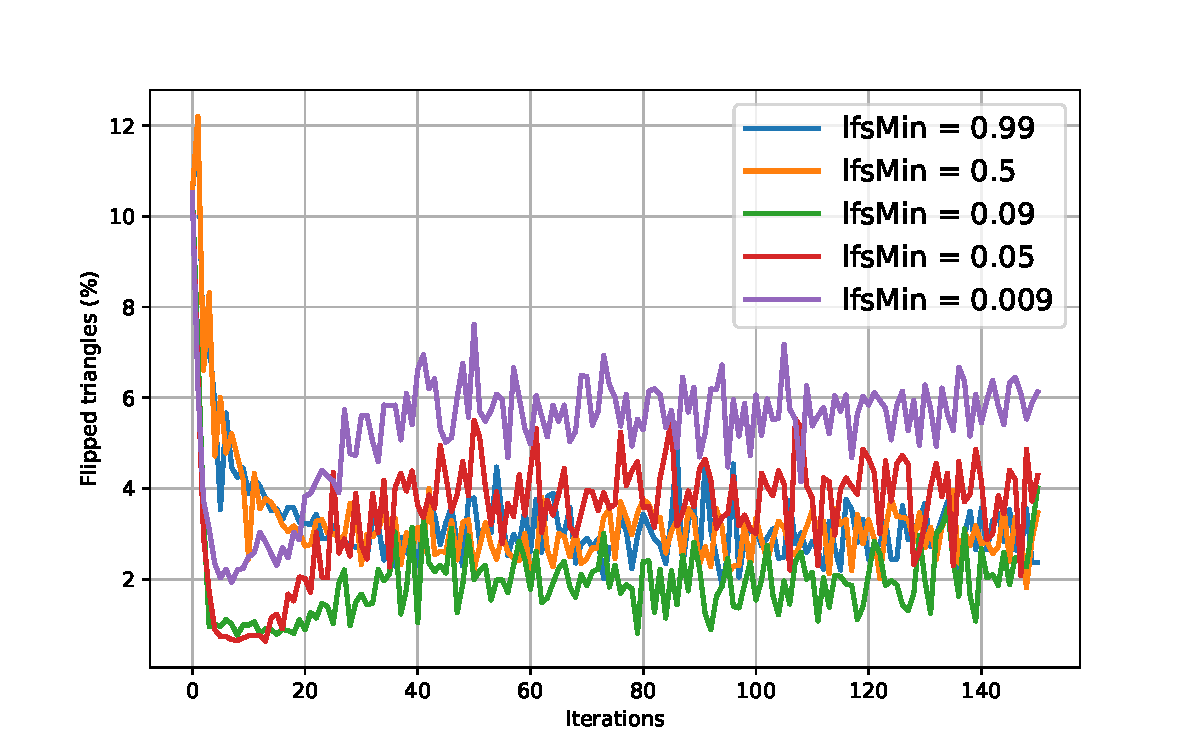
\includegraphics[width=\linewidth]{images/spot_base_lfs_flipped.pdf}
			\caption{Effect of \texttt{lfsMin} on Spot}
			\label{fig:spot_lfs_flipped_base}
		\end{subfigure}
		\caption{Percentage of flipped triangles during the flow.}
		\label{fig:flipped_base}
	\end{figure}
	
	More filter passes clearly improve the mesh quality, because each filter pass averages the previous estimate over the neighbourhood of a vertex, which reduces the noise of the first pass. The results for \texttt{lfsMin} again show that both too small and too large values are harmful.
	
	\begin{figure}[H]
		\centering
		\begin{subfigure}[t]{0.45\textwidth}
			\centering
			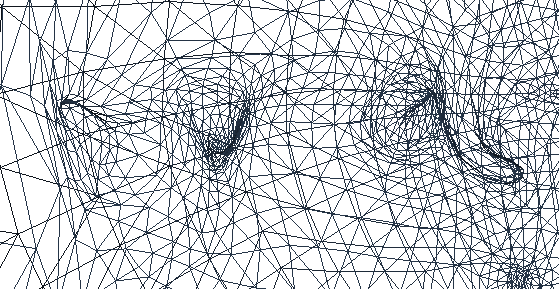
\includegraphics[height=4cm, keepaspectratio]{images/spot_bad_triangles.png}
			\caption{Flipped triangles near the ear of Spot}
		\end{subfigure}
		\hspace{0.05\textwidth}
		\begin{subfigure}[t]{0.45\textwidth}
			\centering
			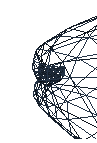
\includegraphics[height=4cm, keepaspectratio]{images/bunny_bad_triangle.png}
			\caption{The ear of the Bunny turned inside out}
		\end{subfigure}
		\caption{Examples of flipped triangles}
		\label{fig:other_flipped_triangles}
	\end{figure}
	
	\paragraph{Conformality.} The cMCF converges to a conformal map, so we also measured how far the map from the initial to the current surface is from conformal. For every triangle, we computed the ratio of the singular values of the linear map from the initial to the current triangle, which is $1$ for a conformal map, and compared it with the deterministic flow. On Spot at $t = 0.1$, $9.6\%$, $12.7\%$ and $15.6\%$ of the triangles are stretched by more than $2{:}1$ for $\delta = 5\cdot10^{-3}$, $1\cdot10^{-3}$ and $5\cdot10^{-4}$, while in the deterministic flow almost none are. On the Bunny, this percentage is about $8.5\%$ for all three time steps.
	
	Table~\ref{tab:global_K_lfs} shows that the number of filter passes and \texttt{lfsMin} affect the shape of the triangles and their position in opposite ways. More filter passes reduce the number of stretched triangles but increase the accumulated error, and a large \texttt{lfsMin} gives the largest accumulated error. This suggests that the filters, which average the estimates over a ball of radius $R$, reduce the noise but introduce a systematic deviation that grows with the size of the balls.
	
	\begin{table}[H]
		\centering
		\begin{tabular}{l c c c}
			\hline
			Test & Accumulated error & Median stretch & Stretched $>2{:}1$ \\
			\hline
			$K = 1$ & 3.57\% & 1.44 & 32.6\% \\
			$K = 2$ & 4.24\% & 1.28 & 25.3\% \\
			$K = 3$ & 4.97\% & 1.24 & 19.1\% \\
			$K = 4$ & 5.74\% & 1.24 & 17.9\% \\
			\hline
			\texttt{lfsMin} $= 0.99$  & 10.10\% & 1.30 & 17.9\% \\
			\texttt{lfsMin} $= 0.5$   & 10.27\% & 1.30 & 18.2\% \\
			\texttt{lfsMin} $= 0.09$  & 6.62\%  & 1.23 & 15.0\% \\
			\texttt{lfsMin} $= 0.05$  & 6.13\%  & 1.22 & 16.1\% \\
			\texttt{lfsMin} $= 0.009$ & 5.80\%  & 1.24 & 21.4\% \\
			\hline
			Deterministic flow & -- & 1.10 & 0.0\% \\
			\hline
		\end{tabular}
		\caption{Accumulated error and conformality on Spot with $\delta = 5\cdot10^{-3}$ after 150 iterations ($t = 0.75$). Stretch: ratio of the singular values of the map from the initial to the current triangle ($1$ for a conformal map).}
		\label{tab:global_K_lfs}
	\end{table}
	
	\section{Methods to improve the mesh quality}
	
	In this section, we evaluate two simple strategies against mesh degeneration.
	
	\subsection{Delta cycle}
	
	Instead of a constant time step, the delta cycle repeats a fixed sequence of decreasing time steps. The idea is that the first step of each cycle, with a large $\delta$, makes fast progress, while the following steps, with smaller and smaller values of $\delta$, smooth the mesh. We tested the cycle
	\begin{equation}
		\delta = \{5 \cdot 10^{-3}, 1 \cdot 10^{-3}, 5 \cdot 10^{-4}, 1 \cdot 10^{-4}, 5 \cdot 10^{-5}, 1 \cdot 10^{-5}, 5 \cdot 10^{-6}, 1 \cdot 10^{-6}, 5 \cdot 10^{-7}, 1 \cdot 10^{-7}\}
	\end{equation}
	on Spot. In the figures, the cycle is plotted once per cycle (every 10th iteration) for readability.
	
	\begin{figure}[H]
		\centering
		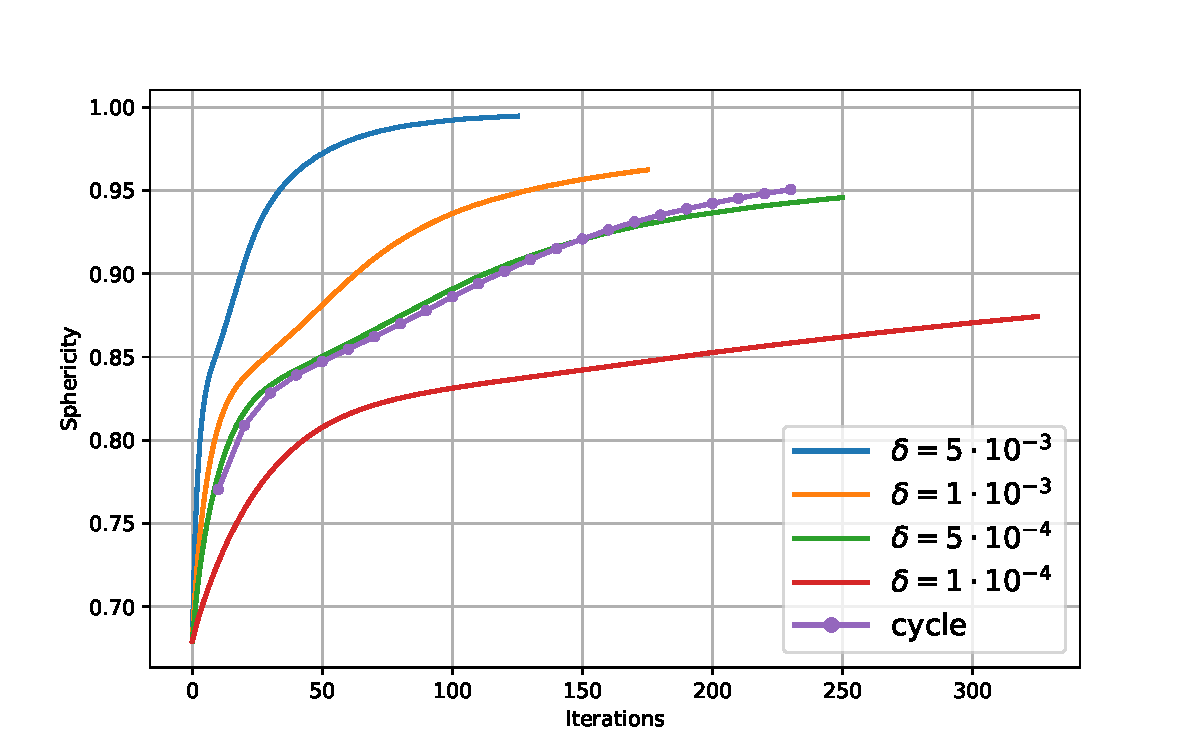
\includegraphics[scale=0.65]{images/spot_cycle_spher.pdf}
		\caption{Sphericity of the delta cycle compared to constant time steps on Spot.}
		\label{fig:spot_cycle_spher}
	\end{figure}
	
	\begin{figure}[H]
		\centering
		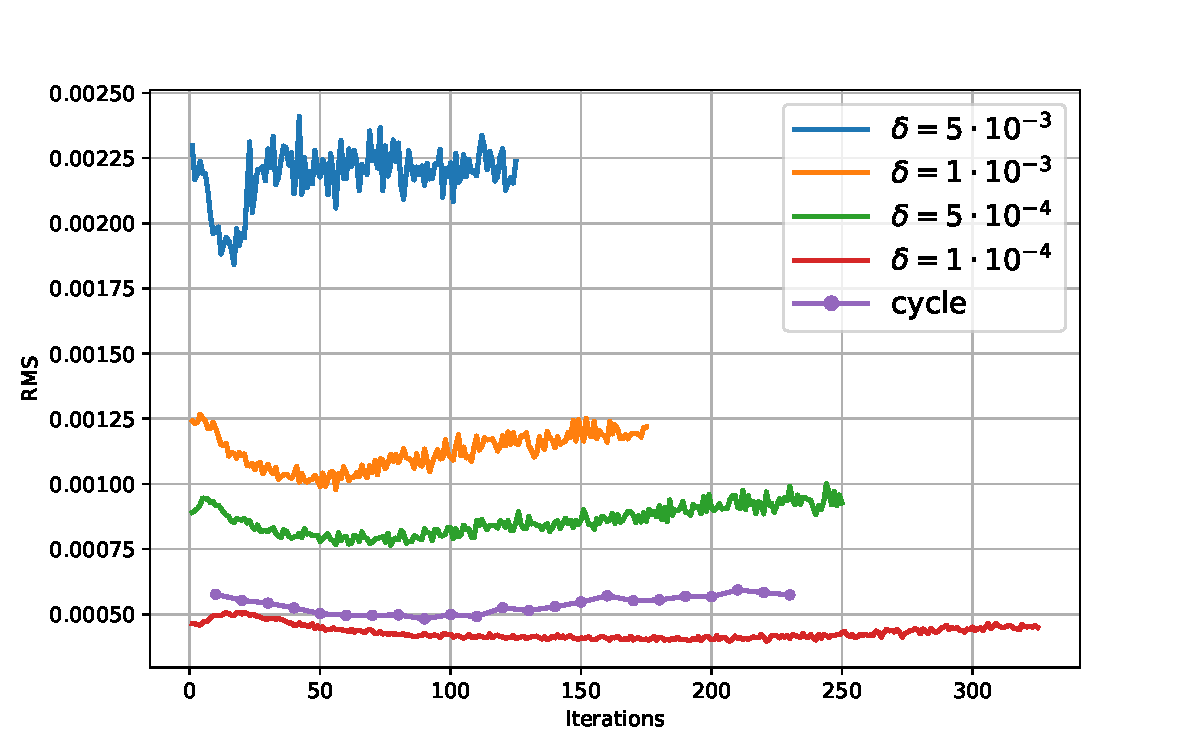
\includegraphics[scale=0.65]{images/spot_cycle_error.pdf}
		\caption{Per-step error of the delta cycle compared to constant time steps on Spot.}
		\label{fig:spot_cycle_error}
	\end{figure}
	
	Both the convergence and the error of the cycle lie between those of the constant time steps, but its running time is very long (Figure~\ref{fig:spot_cycle_time}). The constant time step $\delta = 5 \cdot 10^{-4}$ (green), which reaches a similar sphericity and error, took $3038.7$\,s (50 min 39 s), while the cycle took $7226.6$\,s (2 h 0 min 27 s). The steps with very small $\delta$ are the most expensive, so in this form the delta cycle is not practical.
	
	\begin{figure}[H]
		\centering
		\begin{subfigure}{0.49\textwidth}
			\centering
			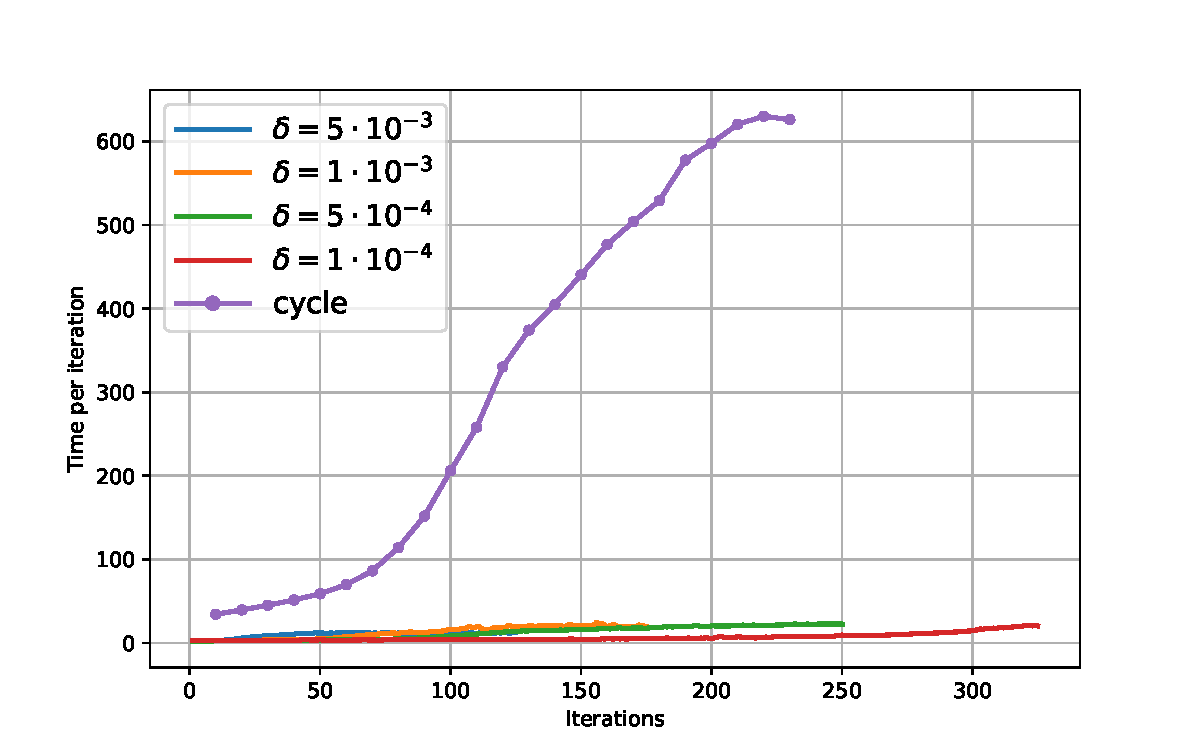
\includegraphics[width=\linewidth]{images/spot_cycle_tpi.pdf}
			\caption{Time per iteration}
		\end{subfigure}
		\hspace{0.00\textwidth}
		\begin{subfigure}{0.49\textwidth}
			\centering
			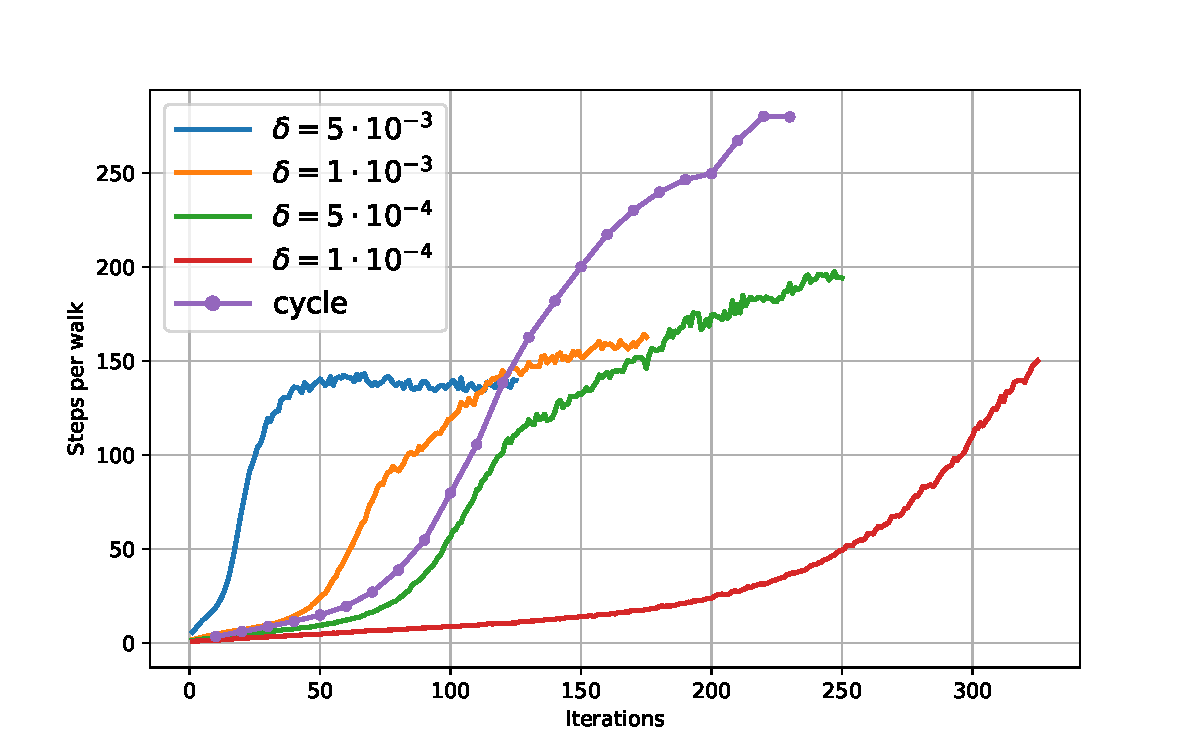
\includegraphics[width=\linewidth]{images/spot_cycle_spw.pdf}
			\caption{Steps per walk}
		\end{subfigure}
		\caption{Running time of the delta cycle compared to constant time steps on Spot.}
		\label{fig:spot_cycle_time}
	\end{figure}
	
	\subsection{Smoothing iterations}
	\label{sec:smoothing}
	
	Based on the observations with the delta cycle, we also tried applying the small time steps only once, at the end of the flow: we continued each constant-$\delta$ run on Spot with a few iterations with decreasing time steps,
	\begin{equation}
		\delta = \{5 \cdot 10^{-4}, 5 \cdot 10^{-5}, 5 \cdot 10^{-6}, 5 \cdot 10^{-7}, 5 \cdot 10^{-8}, 5 \cdot 10^{-9}\}
	\end{equation}
	\begin{figure}[H]
		\centering
		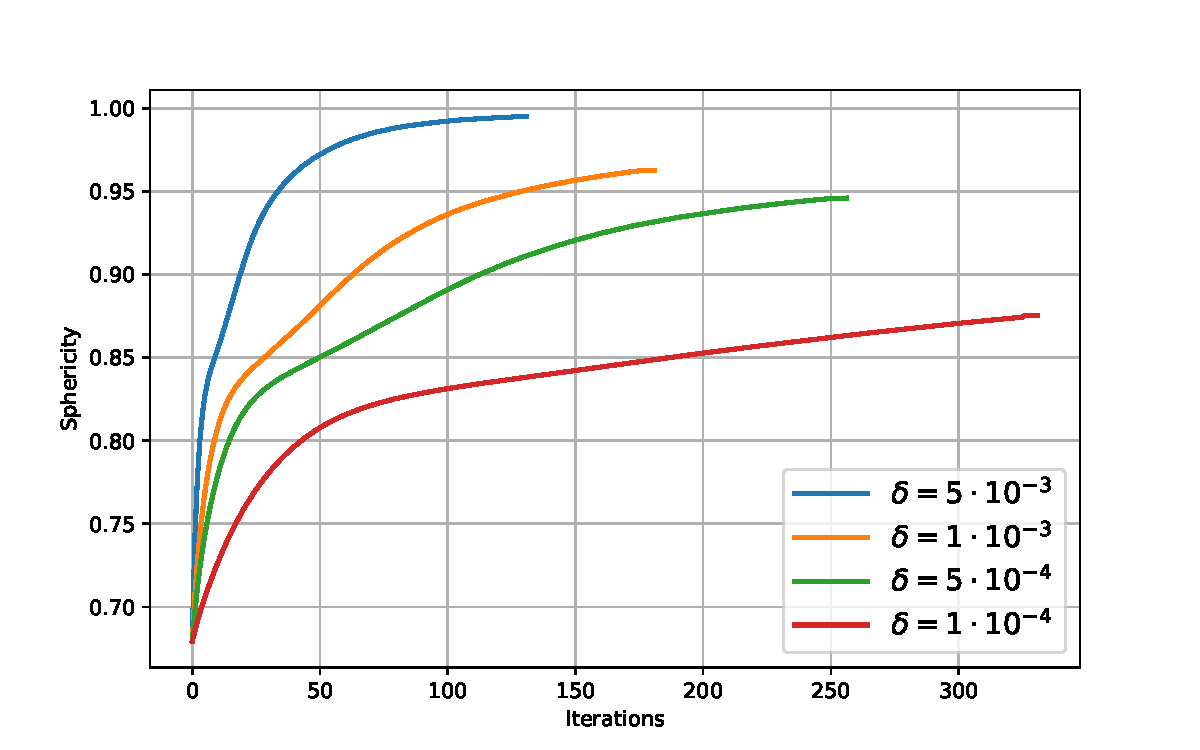
\includegraphics[scale=0.65]{images/spot_repaired_delta_spher.pdf}
		\caption{Sphericity before and after the smoothing iterations on Spot.}
		\label{fig:spot_r_spher}
	\end{figure}
	\begin{figure}[H]
		\centering
		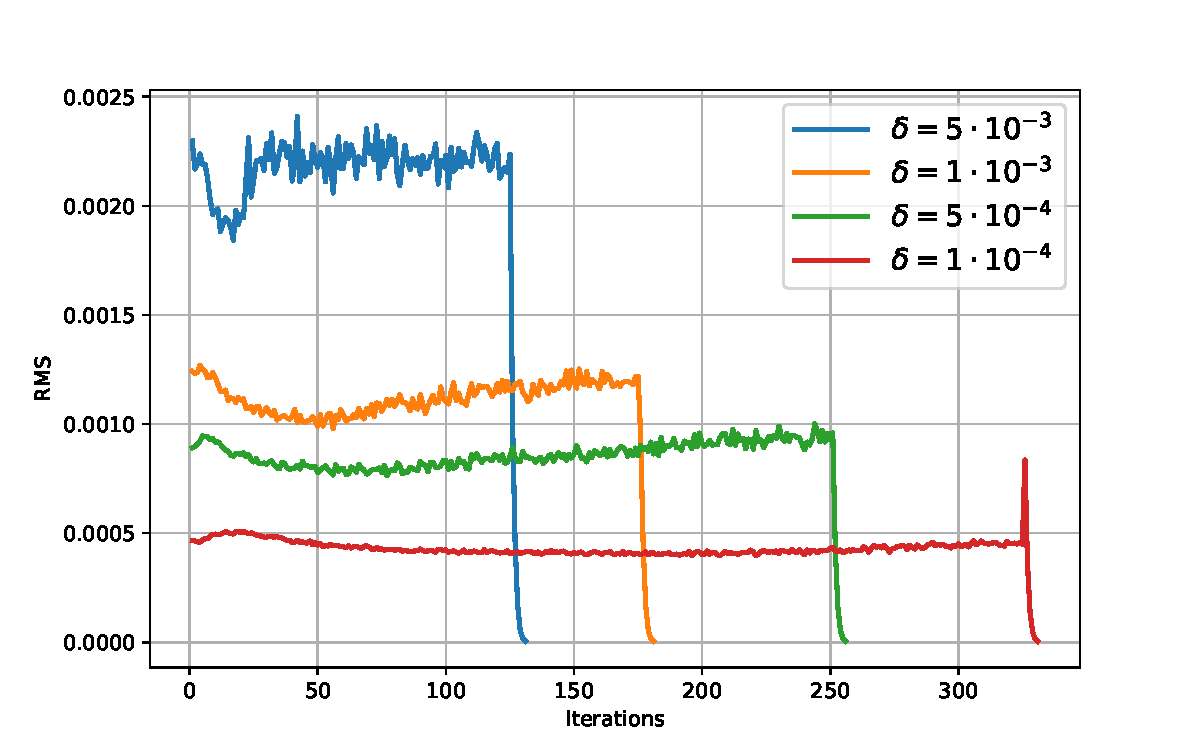
\includegraphics[scale=0.65]{images/spot_repaired_delta_error.pdf}
		\caption{Per-step error before and after the smoothing iterations on Spot.}
		\label{fig:spot_r_error}
	\end{figure}
	
	The smoothing iterations do not reduce the sphericity (Figure~\ref{fig:spot_r_spher}), and their per-step error stays low despite the degraded input mesh (Figure~\ref{fig:spot_r_error}). The drop of the error to almost zero at the end only reflects that a step with a very small $\delta$ barely moves the surface. At the same time, the smoothing iterations repair the degraded triangles very effectively: on Spot with $\delta = 5\cdot10^{-3}$, the minimum angle increases from $0.46^\circ$ to $7.58^\circ$ (Figures~\ref{fig:spot_r_mindeg} and~\ref{fig:smoothing}).
	
	\begin{figure}[H]
		\centering
		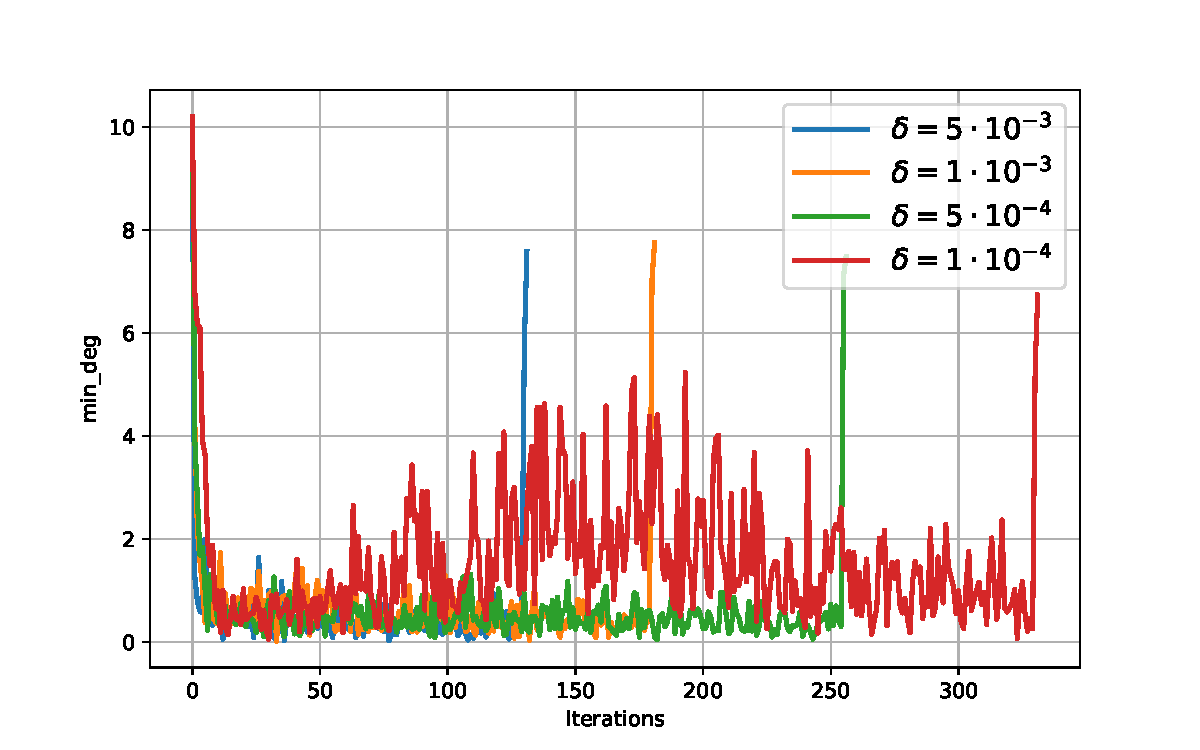
\includegraphics[scale=0.65]{images/spot_repaired_delta_mindeg.pdf}
		\caption{Minimum angle before and after the smoothing iterations on Spot.}
		\label{fig:spot_r_mindeg}
	\end{figure}
	
	\begin{figure}[H]
		\centering
		\begin{subfigure}{0.49\textwidth}
			\centering
			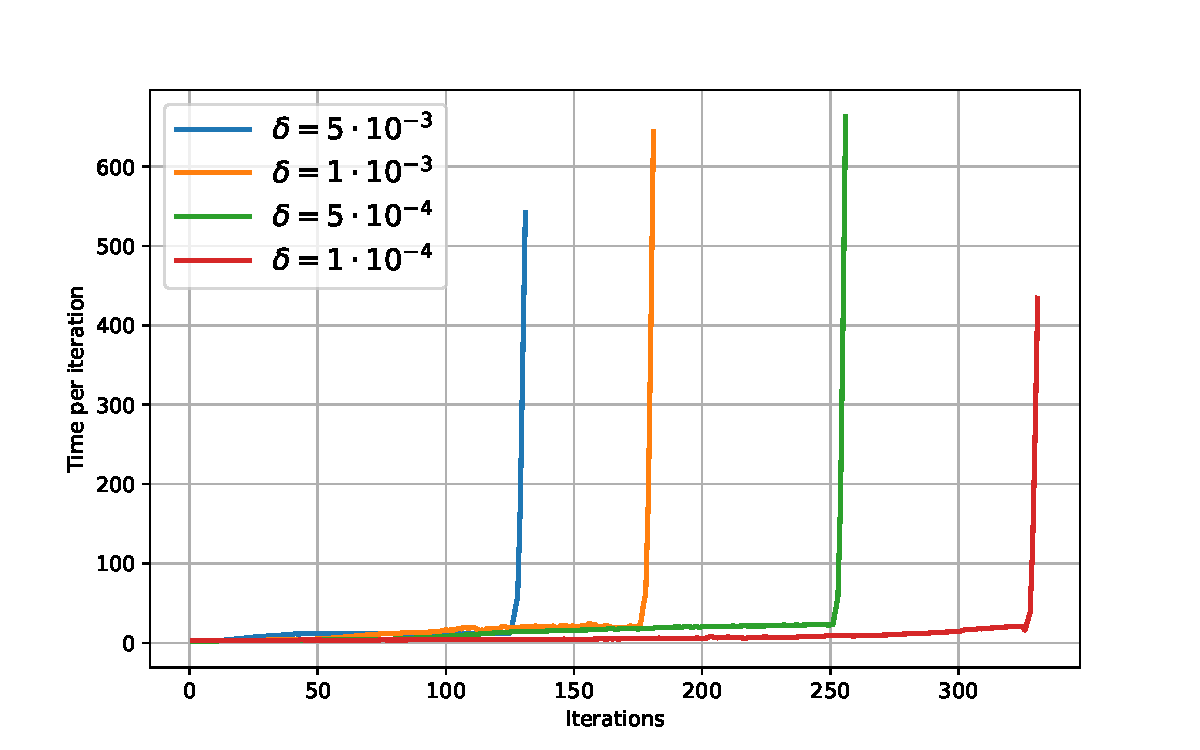
\includegraphics[width=\linewidth]{images/spot_repaired_delta_tpi.pdf}
			\caption{Time per iteration}
		\end{subfigure}
		\hspace{0.00\textwidth}
		\begin{subfigure}{0.49\textwidth}
			\centering
			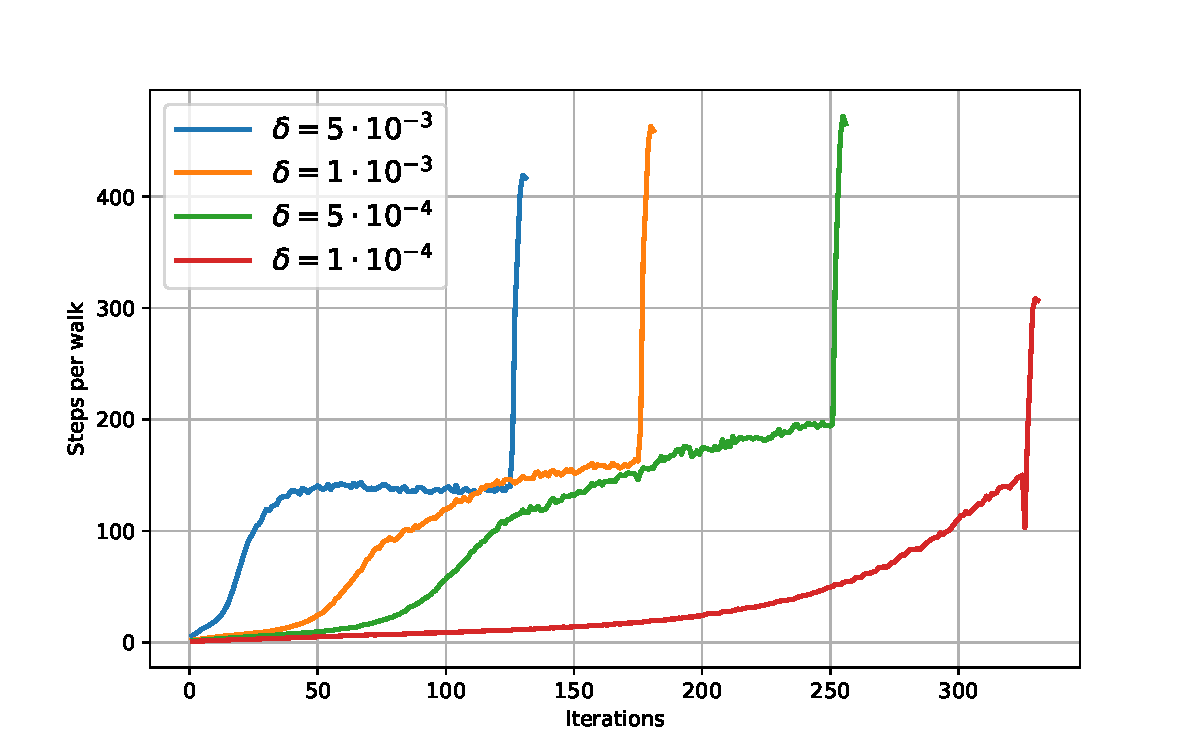
\includegraphics[width=\linewidth]{images/spot_repaired_delta_spw.pdf}
			\caption{Steps per walk}
		\end{subfigure}
		\caption{Running time of the smoothing iterations on Spot.}
		\label{fig:spot_smoothing_time}
	\end{figure}
	
	The smoothing iterations are also expensive, but much cheaper than the cycle. On Spot with $\delta = 5 \cdot 10^{-3}$, the flow itself took $1248.1$\,s (20 min 48 s) and the smoothing $1184.1$\,s (19 min 44 s), about 40 minutes in total, compared to two hours for the delta cycle. The result is also better, because the smoothing is applied to a surface that is already nearly spherical. The last two steps take $892$\,s, $75\%$ of the smoothing time, but they only reduce the percentage of stretched triangles from $4.0\%$ to $2.2\%$ (Table~\ref{tab:smoothing_steps}), so dropping them would cut the cost of the smoothing by a factor of four.
	
	\begin{figure}[H]
		\centering
		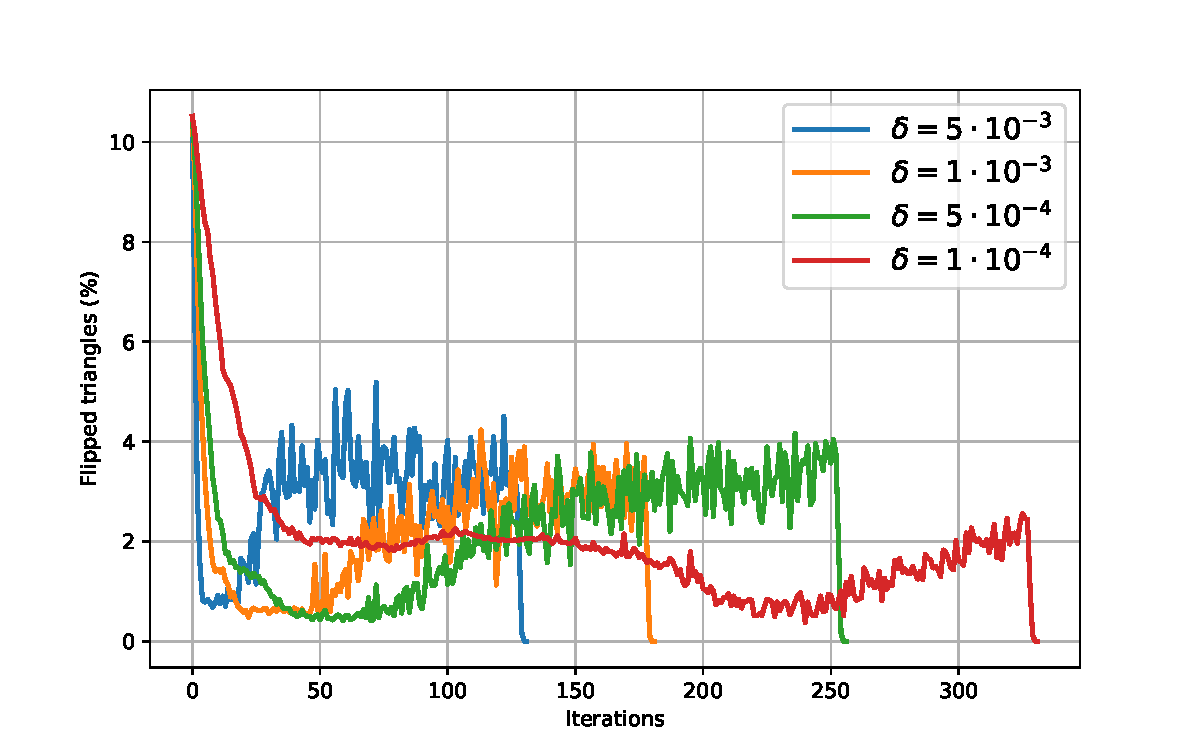
\includegraphics[scale=0.65]{images/spot_repaired_flipped.pdf}
		\caption{Percentage of flipped triangles before and after the smoothing iterations on Spot.}
		\label{fig:spot_r_flipped}
	\end{figure}
	Figure~\ref{fig:spot_r_flipped} shows that the smoothing removes all flipped triangles: at the end of every test, no triangle is flipped.
	\begin{figure}[H]
		\centering
		\begin{subfigure}{0.4\textwidth}
			\centering
			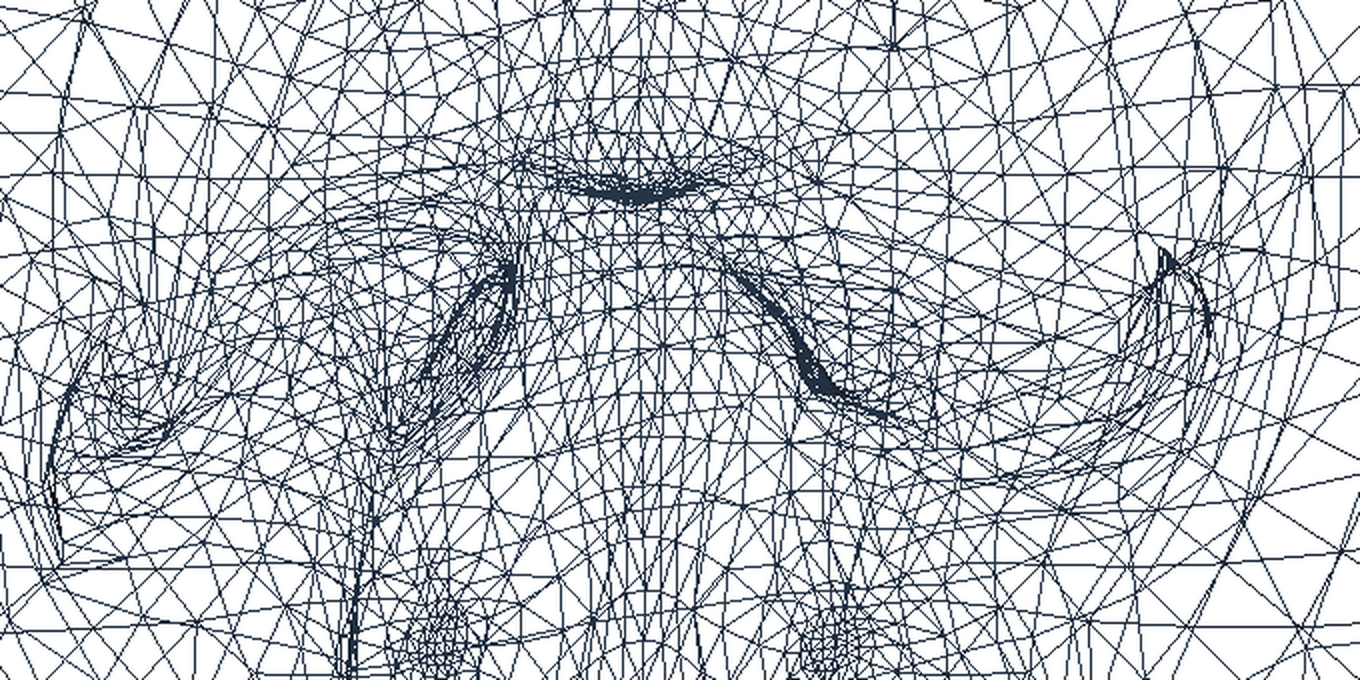
\includegraphics[width=\linewidth]{images/frame_0125_0.png}
			\caption{Iteration 125}
		\end{subfigure}
		\hspace{0.00\textwidth}
		\begin{subfigure}{0.4\textwidth}
			\centering
			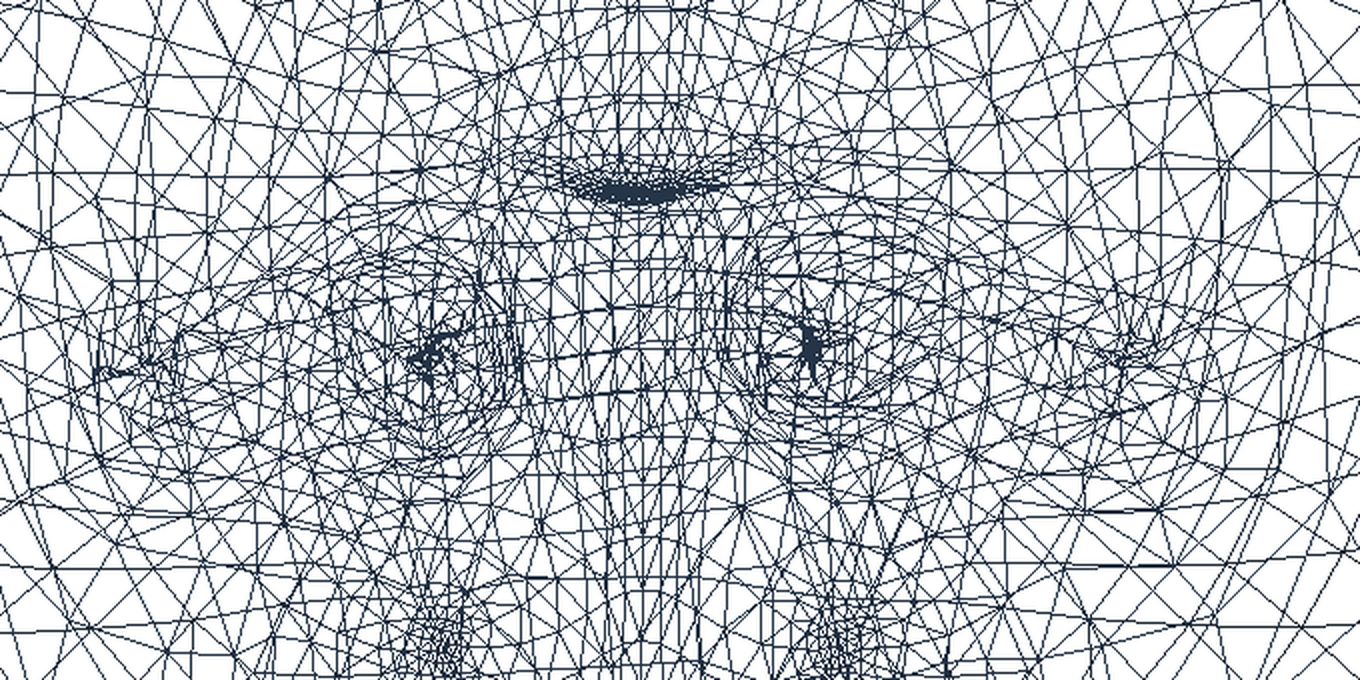
\includegraphics[width=\linewidth]{images/frame_0128_3.png}
			\caption{Iteration 128}
		\end{subfigure}
		\vspace{1em}
		\begin{subfigure}{0.4\textwidth}
			\centering
			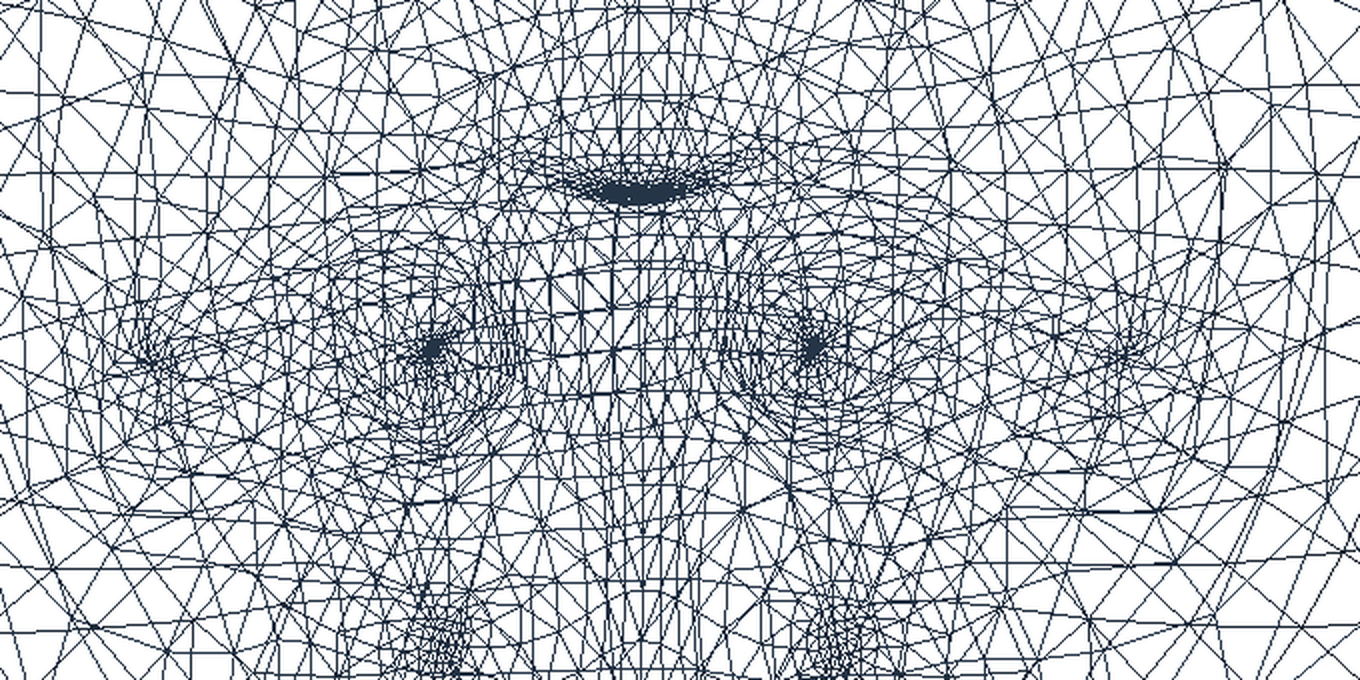
\includegraphics[width=\linewidth]{images/frame_0130_5.png}
			\caption{Iteration 130}
		\end{subfigure}
		\hspace{0.00\textwidth}
		\begin{subfigure}{0.4\textwidth}
			\centering
			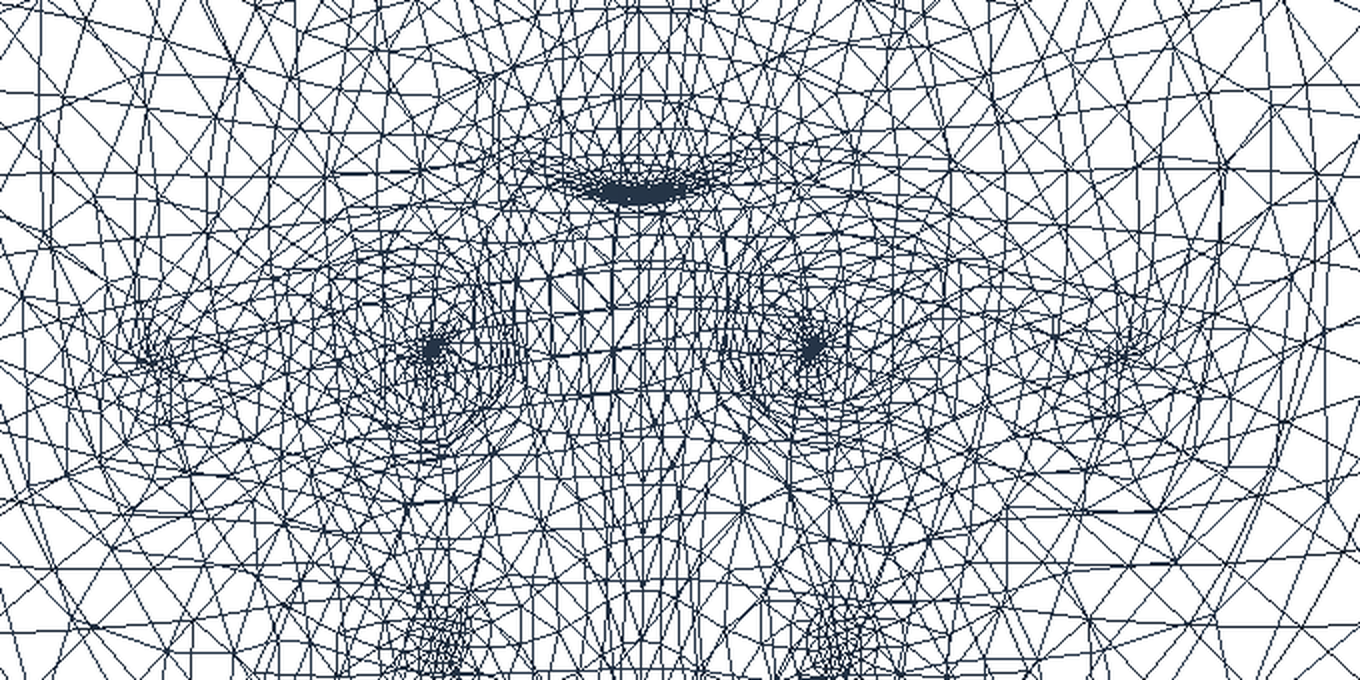
\includegraphics[width=\linewidth]{images/frame_0131_6.png}
			\caption{Iteration 131}
		\end{subfigure}
		
		\caption{The mesh of Spot before (iteration 125) and during the smoothing iterations.}
		\label{fig:smoothing}
	\end{figure}
	
	Table~\ref{tab:smoothing_steps} shows the effect of the individual smoothing steps. Most of the improvement happens in the steps with $\delta = 5\cdot10^{-6}$ and $5\cdot10^{-7}$, where the percentage of stretched triangles drops from $14.3\%$ to $4.0\%$. In these steps, the deterministic flow barely moves the surface, so the repair is most likely caused by the estimator itself: the walks terminate almost immediately, and the filter averages the positions over a small neighbourhood of each vertex. Accordingly, the smoothing improves the shape of the triangles, but not their position: the accumulated error stays at $5.4\%$.
	
	\begin{table}[H]
		\centering
		\small
		\begin{tabular}{r c r c c c}
			\hline
			Iter. & $\delta$ & Time (s) & Median stretch & Stretched $>2{:}1$ & Accumulated error \\
			\hline
			125 & --              & --    & 1.24 & 16.2\% & 5.39\% \\
			126 & $5\cdot10^{-4}$ & 23.9  & 1.22 & 14.2\% & 5.41\% \\
			127 & $5\cdot10^{-5}$ & 40.6  & 1.22 & 14.3\% & 5.41\% \\
			128 & $5\cdot10^{-6}$ & 58.6  & 1.20 & 9.0\%  & 5.41\% \\
			129 & $5\cdot10^{-7}$ & 169.4 & 1.19 & 4.0\%  & 5.42\% \\
			130 & $5\cdot10^{-8}$ & 349.7 & 1.19 & 2.5\%  & 5.42\% \\
			131 & $5\cdot10^{-9}$ & 542.0 & 1.19 & 2.2\%  & 5.42\% \\
			\hline
		\end{tabular}
		\caption{Effect of the individual smoothing iterations on Spot after the flow with $\delta = 5\cdot10^{-3}$. In the deterministic flow, the median stretch is $1.12$, and no triangle is stretched by more than $2{:}1$.}
		\label{tab:smoothing_steps}
	\end{table}
	
	\section{Bonus: cMCF on surfaces of higher genus}
	\label{sec:genus}
	\begin{figure}[H]
		\centering
		\begin{subfigure}{0.3\textwidth}
			\centering
			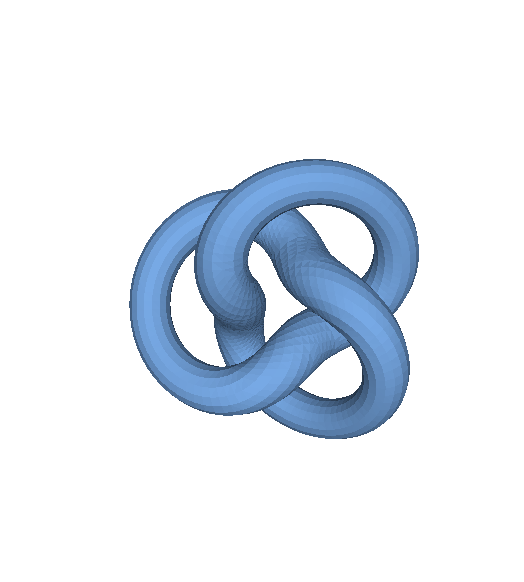
\includegraphics[width=\linewidth]{images/knot_frame_0000.png}
		\end{subfigure}
		\begin{subfigure}{0.3\textwidth}
			\centering
			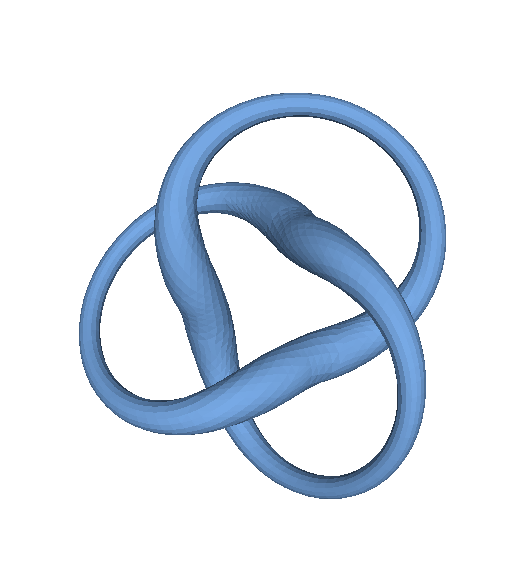
\includegraphics[width=\linewidth]{images/knot_frame_0040.png}
		\end{subfigure}
		\begin{subfigure}{0.3\textwidth}
			\centering
			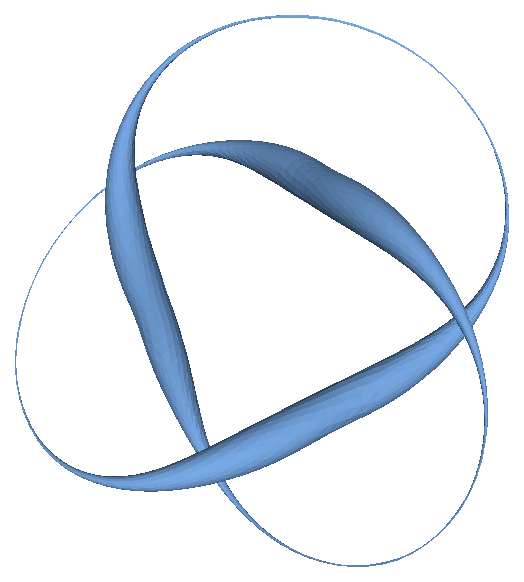
\includegraphics[width=\linewidth]{images/knot_frame_0107.png}
		\end{subfigure}
		\caption[cMCF on the genus-1 Knot model]{cMCF on the genus-1 model Knot (\texttt{1-cgal}) \cite{tuealga_meshes}}
		\label{fig:knot}
	\end{figure}
		
	\begin{figure}[H]
		\centering
		\begin{subfigure}{0.3\textwidth}
			\centering
			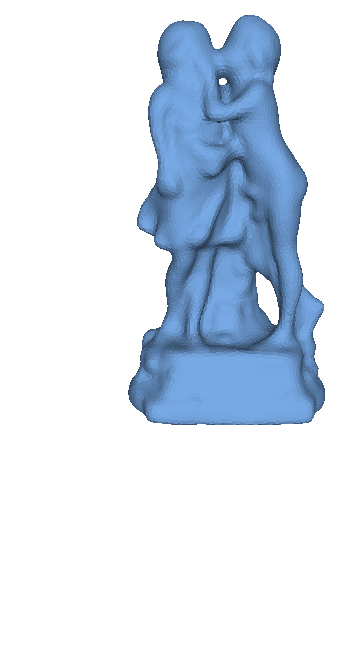
\includegraphics[width=\linewidth]{images/kiss_frame_0000.png}
		\end{subfigure}
		\begin{subfigure}{0.3\textwidth}
			\centering
			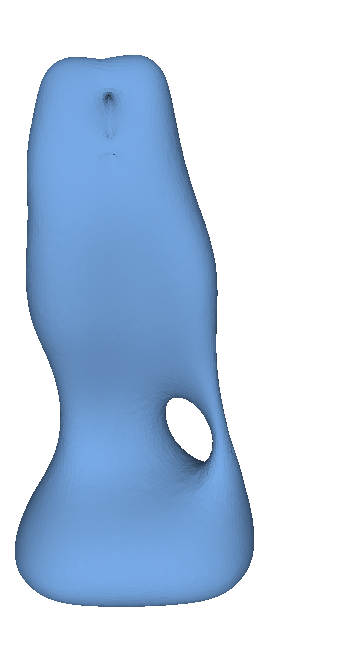
\includegraphics[width=\linewidth]{images/kiss_frame_0005.png}
		\end{subfigure}
		\begin{subfigure}{0.3\textwidth}
			\centering
			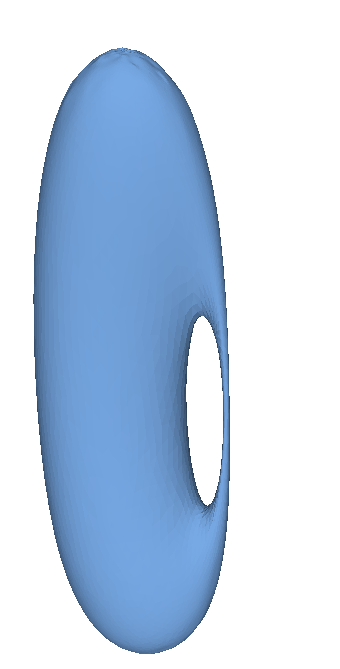
\includegraphics[width=\linewidth]{images/kiss_frame_0060.png}
		\end{subfigure}
		\caption[cMCF on the genus-3 Kiss model]{cMCF on the genus-3 model Kiss (\texttt{gao}) \cite{tuealga_meshes}}
		\label{fig:genusnon0}
	\end{figure}
	
	The cMCF is defined for any closed surface, but only a genus-zero surface can become a sphere. Figures~\ref{fig:knot} and~\ref{fig:genusnon0} show what happens to surfaces of higher genus. The Knot (genus 1) flattens into a thin ribbon: its minimum angle drops from $24.6^\circ$ to $0.02^\circ$ by iteration 107. The Kiss (genus 3) quickly loses its details and becomes a torus-like shape. In both cases, the flow keeps running, but it moves towards a degenerate surface, not towards a sphere.

	
	
	% =====================================================================
	% 7. DISCUSSION AND SUMMARY
	% =====================================================================
	\chapter{Discussion and conclusion}
	\label{ch:summary}

	\section{Future work}
	
	Although the cMCF can be solved with WoS, the noise of the Monte Carlo estimates damages the quality of the mesh. We see several directions that could address this.
	
	The first is an \textit{adaptive time step}. Since $\delta$ strongly affects both the speed of the flow and the quality of the mesh, it could be chosen adaptively: the flow could start with a small $\delta$, increase it while the shape changes slowly and the estimated error is small, and decrease it when the error or the degradation of the mesh grows. Note that a smaller $\delta$ reduces the absolute error of a step, but not necessarily the error relative to the displacement of the step, so the criterion has to be chosen carefully.
	
	The second is a \textit{local majorant}. As the surface approaches the sphere, the area ratio, and therefore $\sigma$, varies strongly over the surface. With the global majorant $\bar{\sigma} = \max \sigma$, the probability $p = \sigma / \bar{\sigma}$ of a real collision is very small in most regions, so most collisions are null collisions, which only make the walks longer (Section~\ref{sec:method-rr}). Delta tracking only requires $\bar{\sigma} \ge \sigma$ inside the current ball, so the majorant can be chosen locally, for example, as the maximum of $\sigma$ over the vertices near the centre of the ball. This requires neither a partition of the surface into regions nor boundaries between them: the walks can move freely, and only the majorant used in each step changes.
	
	The third direction is a different surface walk. PWoS requires a medial axis, a lower bound on the ball radius and a closest-point query in every step, and the closest-point queries dominate the running time. A walk that stays on the surface, for example a random walk along the edges of the mesh, could avoid these costs; developing such a method is left for future work. Finally, the walks are independent, so the solver could be parallelized on the GPU, and the sequence of smoothing steps could be shortened, since the last two steps contribute little to the repair (Table~\ref{tab:smoothing_steps}).
	
	\section{Summary}
	
	We presented a Monte Carlo method for the conformalized mean curvature flow based on Walk on Spheres. The key observation is that the operator of the cMCF is defined with respect to the metric of the initial surface, so after a semi-implicit time discretization every step is a screened Poisson equation on the fixed original surface, with a spatially varying screening coefficient. We solved these equations with projected walks on spheres and delta tracking, and reduced the noise with mean value filtering and antithetic walk pairs. The method makes genus-zero surfaces converge to the sphere, but the noise degrades the mesh; a few final iterations with decreasing time steps repair the mesh at a moderate cost.
	
	The method is much slower than a deterministic solver of the same discretization, which solves one sparse linear system per step (Table~\ref{tab:time_of_tests}). Its advantages are that it needs no linear system, the solution can be evaluated at individual points, and the walks are independent, so it is trivially parallelizable, which could reduce the running time considerably. More generally, the same approach applies to geometric flows whose operator is defined on a fixed reference surface.
	
	
	% Acknowledgements (optional)
	\chapter*{\acklabel}
	\addcontentsline{toc}{chapter}{\acklabel}
	I would like to thank my advisor, Dr. Fábián Gábor, for introducing me to this topic and for the constant support he has given in the making of this paper. 
	
	% Appendices (optional)
	\appendix
	
	\chapter{Supplemental Notes}
	\label{app:supplemental}	
	
	\section{The coefficient $c_r$ of the screened mean value formula}
	\label{app:cr}
	
	\paragraph{Step 1: $c_r$ is the total weight of the boundary term.}
	By Green's second identity, the boundary term of the representation formula is
	$\int_{\partial B} P(y)\,u(y)\,dy$, where $P=-\partial_n G^{\sigma}_r(x,\cdot)$
	is the Poisson kernel of the ball. The ball and the equation are invariant
	under rotations around the center $x$, so $P$ is constant on $\partial B$.
	Hence
	\begin{equation}
		\int_{\partial B} P\,u\,dy = \Big(\int_{\partial B}P\,dy\Big)\frac{1}{|\partial B|}\int_{\partial B}u\,dy,
		\qquad\text{so}\qquad c_r=\int_{\partial B}P\,dy .
	\end{equation}
	
	\paragraph{Step 2: a test problem that isolates $c_r$.}
	Let $h$ solve the homogeneous problem
	\begin{equation}
		(\Delta-\sigma)h=0 \ \text{in } B,\qquad h=1 \ \text{on } \partial B .
	\end{equation}
	Since $f=0$ and the boundary data is $1$, formula \eqref{theint} gives
	$h(x)=c_r\cdot 1$, that is,
	\begin{equation}
		c_r = h(x).
	\end{equation}
	(For $\sigma>0$ the maximum principle makes the solution unique, so any solution we
	find below is \emph{the} solution.)
	
	\paragraph{Step 3: solving for $h$.}
	By symmetry $h=h(\rho)$ with $\rho=\|y-x\|$. Let $s=\sqrt{\sigma}$. The Laplacian of a radial function in
	$\mathbb{R}^3$ is $h''+\frac{2}{\rho}h'$, so
	\begin{equation}
		h''+\frac{2}{\rho}h'-s^2h=0 .
	\end{equation}
	Substituting $w(\rho)=\rho\,h(\rho)$ gives $w''=\rho h''+2h'$, hence
	$w''-s^2w=0$ and
	\begin{equation}
		h(\rho)=\frac{A\sinh(s\rho)+B\cosh(s\rho)}{\rho}.
	\end{equation}
	$h$ must be bounded at $\rho=0$, which forces $B=0$. The boundary condition
	$h(r)=1$ gives $A\sinh(sr)/r=1$, so $A=r/\sinh(sr)$ and
	\begin{equation}
		h(\rho)=\frac{r}{\sinh(sr)}\,\frac{\sinh(s\rho)}{\rho}.
	\end{equation}
	
	\paragraph{Step 4: value at the center.}
	Since $\sinh(s\rho)/\rho\to s$ as $\rho\to 0$,
	\begin{equation}
		c_r=h(0)=\frac{rs}{\sinh(sr)}=\frac{\kappa}{\sinh\kappa},
		\qquad \kappa=r\sqrt{\sigma}.
	\end{equation}

	
	% Bibliography (mandatory)
	\cleardoublepage
	\phantomsection
	\addcontentsline{toc}{chapter}{\biblabel}
	\printbibliography[title=\biblabel]
	
	% Lists (keep only the ones you actually fill with content)
	\cleardoublepage
	\phantomsection
	\addcontentsline{toc}{chapter}{\lstfigurelabel}
	\listoffigures
	
	\cleardoublepage
	\phantomsection
	\addcontentsline{toc}{chapter}{\lstalgorithmlabel}
	\listofalgorithms
	
	\cleardoublepage
	\phantomsection
	\addcontentsline{toc}{chapter}{\lsttablelabel}
	\listoftables
	
	\cleardoublepage
	\phantomsection
	\chapter*{Use of Artificial Intelligence}
	\addcontentsline{toc}{chapter}{Use of Artificial Intelligence}
	
	In the making of this paper, artificial intelligence usage was reduced only for this two cases:
	\begin{enumerate}
		\item \textbf{Picture generation}: The illustration presented in Figure~\ref{fig:wos_example} was generated using Sonnet 5.5 (Anthropic).
		\item \textbf{Language and grammar checking}: Sonnet 5.5 (Anthropic) and \href{https://app.grammarly.com/}{Grammarly} were used.
	\end{enumerate}
	
	\cleardoublepage
	\phantomsection
	\chapter*{Statement of results}
	\addcontentsline{toc}{chapter}{Statement of results}
	
	The main topic, conformalized mean curvature flow was introduced to me by my advisor, Dr. Fábián Gábor. He gathered the literature that I used to start working the problem. The other main topic of this paper was the Walk on Spheres method. This was also introduced to me by Gábor and we worked with this method earlier this year. We discussed many ways to approach the problem of how could we write up the conformalized mean curvature flow, so that the Walk on Spheres method can solve it. The idea we agreed on was mine. I also implemented the solver, the visualization which was used to showcase how the geometry evolves, and the the tester. The making of this paper, including the writing of it, the original design, making of the figures and graphs was also done by me, and Gábor helped me with formalizing the paper and pointed out errors to me. 
	
	
	%\cleardoublepage
	%\phantomsection
	%\addcontentsline{toc}{chapter}{\lstcodelabel}
	%\lstlistoflistings
	
	% List of symbols (needs an extra makeindex run; the notation table in
	% Section~\ref{sec:notation} is an easier alternative)
	%\printnomenclature
	
\end{document}